\documentclass[defaultstyle,10pt,master,Arial]{ISTthesisEN}
% Use ISTthesisPT for portuguese version 

\input{beg-definitions/packages.tex}
\input{beg-definitions/pagesetup.tex}

\begin{document}

\onehalfspacing
\selectlanguage{english}

\pagestyle{begin}
\input{beg-firstFewPages/1.Cover.tex} 
\thispagestyle{empty}
\hbox{} \vfill
\begin{flushright}
\small \textit{\textbf{The behavior of large and complex aggregates of elementary particles, it turns out, is not to be understood in terms of a simple extrapolation of the properties of a few particles.}}
\\ \vspace{2mm}  
\scriptsize P. W. Anderson
\\ \vspace{10mm}  
Cover picture credit: University of Manchester \\
\url{www.graphene.manchester.ac.uk} (accessed on 12 June 2018)
\end{flushright}

\clearpage
\thispagestyle{empty}
\cleardoublepage

\pdfbookmark{Acknowledgments}{Acknowledgments}
\begin{acknowledgments} 

I would like to thank my supervisors Prof. Eduardo Filipe Vieira de Castro, and Prof. João Manuel Viana Parente Lopes

\end{acknowledgments}
\clearpage
\thispagestyle{empty}
\cleardoublepage
\selectlanguage{english}
\begin{abstract}

The aim of this work (English)

\end{abstract}
\begin{keywords}
Hubbard Model, Strongly Correlated Electrons, \aclp{TMD}, \acf{QMC} (English)
\end{keywords}
\clearpage
\thispagestyle{empty}
\cleardoublepage
\selectlanguage{portuguese}
\begin{resumo}

O comportamento coletivo tem estado na linha da frente da investigação feita em física da matéria condensada durante grande parte do último século.
Esta era dos sistemas complexos trouxe-nos um conceito denominado emergência que tem, atualmente, uma natureza transversal.
Em particular, em sistemas de eletrões fortemente correlacionados, fenómenos emergentes conduzem a uma enorme variedade de propriedades exóticas que desafiam a intuição.

A descoberta de materiais bidimensionais renovou o interesse no problema a $N$ eletrões dado que as interações eletrão-eletrão têm um papel determinante na descrição de muitas das propriedades destes sistemas.
Além disso, o rápido aumento de poder computacional e de sofisticação algorítmica tornou possível atacar problemas que eram até então inacessíveis.
Neste trabalho, focamo-nos numa classe particular de materiais bidimensionais, mostrando uma grande riqueza de propriedades óticas e eletrónicas: os dicalcogenetos de metais de transição.

Neste contexto, investigamos a emergência de magnetismo associado a estados de fronteira, num tipo de nanoestrutura chamado de nanofita, dada a sua semelhança a uma fita, por ser muito mais longa numa direção que na outra.
Para estudar este fenómeno, consideramos um modelo de tight-binding baseado em considerações de simetria que captura a maioria das propriedades relacionadas com a \say{física de fronteiras} do problema.
Depois, generalizamos este modelo para o caso interatuante, considerando interações do tipo Hubbard intra-orbitais.

A nossa abordagem ao problema divide-se em duas partes.
Começamos por levar a cabo cálculos numéricos originais na aproximação de campo médio para construir uma imagem física aproximada do sistema.
Depois, usamos a nossa própria implementação de um algoritmo de ponta, livre de enviesamento estatístico - o método do determinante de Monte Carlo Quântico - para simular o sistema interatuante a $N$ fermiões em estudo.
\end{resumo}
\vspace{-2.5cm}
\begin{palavraschave}
Materiais Bidimensionais, Modelo de Hubbard, Eletrões Fortemente Correlacionados, Nanofitas de Dicalcogenetos de Metais de Transição, Teoria de Campo Médio, Monte Carlo Quântico: Método do Determinante ou Campo Auxiliar (Português)
\end{palavraschave}
\clearpage
\thispagestyle{empty}
\cleardoublepage
\selectlanguage{english}
\input{beg-firstFewPages/6.Tables.tex}
\acresetall
% Remember that in the list of tables titles are set manually
% %%%%%%%%%%%%%%%%%%%%%%%%%%%%%%%%%%%%%%%%%%%%%%%%%%%%%%%%%%%%%%%%%%%%%%
 % List of acronyms
\pdfbookmark[1]{List of Acronyms}{loac}

\chapter*{Abbreviations}


% See more at http://staff.science.uva.nl/~polko/HOWTO/LATEX/acronym.html

\begin{acronym}
%\acro{acro}{Dummy Acronym}
\acro{QMC}{Quantum Monte Carlo}
\acro{TMD}{Transition Metal Dichalcogenide}
\acro{LG}{Landau Ginzburg}
\end{acronym}


%\ac{acro} 
% The first time you use this, the acronym will be written in full with the acronym in parentheses: supernova (SN). At later times it will just print the acronym: SN.

%\acf{acro}
% written out form with acronym in parentheses, irrespective of previous use

%\acs{acro}
% acronym form, irrespective of previous use

%\acl{acro}
% written out form without following acronym

%\acp{acro}
% plural form of acronym by adding an s. \acfp. \acsp, \aclp work as well.

\clearpage
\thispagestyle{empty}
\cleardoublepage




%%%%%%%%%%%%%%%%%%%%%%%%%%%%%%%%%%%%%%%%%%%%%%%%%%%%%%%%%%%%%%%%%%%%%%
% List of symbols
% I'm not using any non standard symbol. I'm simply keeping this so as not to mess up the page numbering.
%\pdfbookmark[1]{List of Symbols}{los}

%\listofsymbols


\clearpage
\thispagestyle{empty}

\cleardoublepage
% Pages number is starting now with arabic style... until now it was on roman mode
\pagenumbering{arabic} \setcounter{page}{1}
\baselineskip 18pt
\selectlanguage{english}
% Define the title of Chapter Table of Contents
\mtcsettitle{minitoc}{Contents}
\pagestyle{documentsimple}%Simple head
% Insert chapters here

\fancychapter{Introduction}
\label{cap:int}

\slshape

The isolation of graphene in 2004 has led to a growing interest of the scientific community in two-dimensional materials revealing extraordinary properties.
In fact, their very existence was not expected a priori because at first sight they seem to violate the Mermin-Wagner-Hohenberg theorem \cite{mermin_absence_1966, coleman_there_1973, hohenberg_existence_1967}, a no-go theorem that forbids ordering below three dimensions at finite temperature.
Since graphene was discovered, a plethora of similarly stable \ac{2D} materials has been discovered.
A vast set of open problems remains to be solved within the realm of their fascinating and counterintuitive properties. These are often tackled by carrying out numerical simulations. \ac{QMC} is a simulation method that is amply applicable to condensed matter physics problems. Despite the system size being constrained due to limited simulation time, reliable and accurate solutions are provided to the otherwise intractable quantum many-body problem. The field is currently very active and method optimization can prove crucial in applications to real physical systems. In this work, \acs{QMC} is used to simulate a two-dimensional system with strong electron interactions giving rise to promising properties: a nanostructure made of a recent member of the \acs{2D} materials family called a nanoribbon.

\normalfont


\section{Strongly correlated electron systems}
\label{sec:strongly_correlated}

Condensed matter physics is concerned with the emergence of the properties of quantum materials from complexity.
The central concept within this approach is that of symmetry breaking.
When a phase transition occurs, a system is said to condense into a phase of lower symmetry.
A simple pictorial example is the transition from a gas to a solid.
Statistically, any point within a gas is equivalent, that is, on average, the surroundings of all points look similar.
Formally, the system is then said to be fully translationally invariant.
On the other hand, in a solid, a point is only equivalent to a discrete set of other points.
In fact, a simplified view of a solid consists of a periodic arrangement of atoms occupying the points of a lattice.
Any point on the lattice can be reached starting from any other point upon translation by a lattice vector.
Thus, a system that makes a transition from the gaseous to the solid state becomes invariant only under a discrete set of translations, rather than a continuous one. 

A framework that is commonly used to identify symmetry breaking is the \ac{LG} theory of phase transitions.
The theory gives a prescription to discover phase transitions.
More precisely, it gives criteria for a symmetry to become manifest.
Although this framework is very useful, it turns out that the search for order relies on symmetry ideas well beyond condensed matter.
Symmetry breaking gives rise to emergent phenomena.
The idea of emergence rests on a constructionist, rather than a reductionist hypothesis: that the behavior of the many does not trivially follow from the behavior of the few.
As P.W. Anderson puts it, \say{The ability to reduce everything to simple fundamental laws does not imply the ability to start from those laws and reconstruct the universe.} \cite{anderson_more_1972}

The broad scope of condensed matter comes from the sheer number of possibilities that the symmetry breaking approach affords.
For the specific case of the \acs{LG} theory, one can study the emergence of magnetism, superconductivity, or superfluidity, just to name a few.
However, as we shall see, sometimes the \acs{LG} theory fails to capture a system's behavior, and we must resort to other theories to identify these, or other eventual properties that might arise.
The \acl{LG} procedure can be summarized as follows: identify an order parameter reflecting the underlying symmetry of the system, and minimize the free energy in order to deduce conditions for the symmetry to become manifest, leading to a phase transition.
The drawback of this approach is that it might be difficult to identify an order parameter in the first place.
Moreover, even if we do manage to find one, the usual procedure may be impossible to perform.
It can easily happen that the degree of complexity of the order parameter is simply too high.
Additionally, and perhaps more importantly, not all phase transitions can be described by the LG paradigm.

On the one hand, there are systems where a different kind of order arises.
A prominent example is that of fractional quantum Hall effect, where (rather surprisingly!) the \emph{quasi-particles} describing the excitations of the quantum Hall fluid carry \emph{fractions} of the electron charge.
There is an intimate connection between charge fractionalization and topology, which may be understood in terms of the properties of the Laughlin states describing the quantum Hall fluid. However, while it is tempting to try to characterize the latter in terms of the \acs{LG} paradigm, it must actually be regarded as a distinct type of matter, where \say{topological order} arises.
The proposal put forward by Wen \cite{wen_topological_1990} rests on characterizing quantum states by their ground state degeneracy, and investigating how they change under operations defined on specific manifolds. 

On the other hand, for the so called strongly correlated systems we shall focus on in this work, there are phenomena which emerge specifically due to the interacting nature of the problem.
They are elusive because a description in terms of the \acs{LG} paradigm does not yield a behavior consistent with what is observed empirically.
Instead, order emerges from the complexity created by the interactions among all the constituents.
The \acs{LG} theory fails because it ignores these interactions by disregarding fluctuations in the microscopic configuration of a system.
This approximation consists of reducing the complex interactions to an effective \emph{mean field}, which is normally determined self consistently.
Strongly correlated systems require an approach beyond mean field, which makes them both extremely interesting and notoriously difficult to tackle.
The mean field view fails to describe them because it considers each constituent to interact only with an external entity representing the interactions with all other constituents, ignoring collective behavior.
In fact, the failure of mean field theory is not limited to correlated systems, and its success in describing a given system depends, for example, on the dimensionality\footnote{Normally, there is an upper critical dimension $d_c$ above which mean field is exact. Below $d_c$, its predictions might be useful qualitatively, but not quantitatively.} and on the range of the particular type of interaction that is considered.

In many cases, mean field theory is too extreme of an approximation.
Nonetheless, its occasional failure at capturing the whole of a system's properties does not deem it  useless.
Actually, it is quite the contrary.
Mean field is often used as a first approach to build an intuitive physical picture for the general properties and behavior of the system.
Of course, this is done while keeping in mind that the description it provides might be intrinsically insufficient.
Clearly, to extract the features of a correlated system we must  extend it to the fully interacting case.
\section{State of The Art}
\label{sec:int_state}



\section{Original Contributions}
\label{sec:int_contributions}

\input{ch-introduction/4.outline.tex}

\cleardoublepage

\fancychapter{Introduction}
\label{cap:int}

\slshape

The isolation of graphene in 2004 has led to a growing interest of the scientific community in two-dimensional materials revealing extraordinary properties.
In fact, their very existence was not expected a priori because at first sight they seem to violate the Mermin-Wagner-Hohenberg theorem \cite{mermin_absence_1966, coleman_there_1973, hohenberg_existence_1967}, a no-go theorem that forbids ordering below three dimensions at finite temperature.
Since graphene was discovered, a plethora of similarly stable \ac{2D} materials has been discovered.
A vast set of open problems remains to be solved within the realm of their fascinating and counterintuitive properties. These are often tackled by carrying out numerical simulations. \ac{QMC} is a simulation method that is amply applicable to condensed matter physics problems. Despite the system size being constrained due to limited simulation time, reliable and accurate solutions are provided to the otherwise intractable quantum many-body problem. The field is currently very active and method optimization can prove crucial in applications to real physical systems. In this work, \acs{QMC} is used to simulate a two-dimensional system with strong electron interactions giving rise to promising properties: a nanostructure made of a recent member of the \acs{2D} materials family called a nanoribbon.

\normalfont


\section{Strongly correlated electron systems}
\label{sec:strongly_correlated}

Condensed matter physics is concerned with the emergence of the properties of quantum materials from complexity.
The central concept within this approach is that of symmetry breaking.
When a phase transition occurs, a system is said to condense into a phase of lower symmetry.
A simple pictorial example is the transition from a gas to a solid.
Statistically, any point within a gas is equivalent, that is, on average, the surroundings of all points look similar.
Formally, the system is then said to be fully translationally invariant.
On the other hand, in a solid, a point is only equivalent to a discrete set of other points.
In fact, a simplified view of a solid consists of a periodic arrangement of atoms occupying the points of a lattice.
Any point on the lattice can be reached starting from any other point upon translation by a lattice vector.
Thus, a system that makes a transition from the gaseous to the solid state becomes invariant only under a discrete set of translations, rather than a continuous one. 

A framework that is commonly used to identify symmetry breaking is the \ac{LG} theory of phase transitions.
The theory gives a prescription to discover phase transitions.
More precisely, it gives criteria for a symmetry to become manifest.
Although this framework is very useful, it turns out that the search for order relies on symmetry ideas well beyond condensed matter.
Symmetry breaking gives rise to emergent phenomena.
The idea of emergence rests on a constructionist, rather than a reductionist hypothesis: that the behavior of the many does not trivially follow from the behavior of the few.
As P.W. Anderson puts it, \say{The ability to reduce everything to simple fundamental laws does not imply the ability to start from those laws and reconstruct the universe.} \cite{anderson_more_1972}

The broad scope of condensed matter comes from the sheer number of possibilities that the symmetry breaking approach affords.
For the specific case of the \acs{LG} theory, one can study the emergence of magnetism, superconductivity, or superfluidity, just to name a few.
However, as we shall see, sometimes the \acs{LG} theory fails to capture a system's behavior, and we must resort to other theories to identify these, or other eventual properties that might arise.
The \acl{LG} procedure can be summarized as follows: identify an order parameter reflecting the underlying symmetry of the system, and minimize the free energy in order to deduce conditions for the symmetry to become manifest, leading to a phase transition.
The drawback of this approach is that it might be difficult to identify an order parameter in the first place.
Moreover, even if we do manage to find one, the usual procedure may be impossible to perform.
It can easily happen that the degree of complexity of the order parameter is simply too high.
Additionally, and perhaps more importantly, not all phase transitions can be described by the LG paradigm.

On the one hand, there are systems where a different kind of order arises.
A prominent example is that of fractional quantum Hall effect, where (rather surprisingly!) the \emph{quasi-particles} describing the excitations of the quantum Hall fluid carry \emph{fractions} of the electron charge.
There is an intimate connection between charge fractionalization and topology, which may be understood in terms of the properties of the Laughlin states describing the quantum Hall fluid. However, while it is tempting to try to characterize the latter in terms of the \acs{LG} paradigm, it must actually be regarded as a distinct type of matter, where \say{topological order} arises.
The proposal put forward by Wen \cite{wen_topological_1990} rests on characterizing quantum states by their ground state degeneracy, and investigating how they change under operations defined on specific manifolds. 

On the other hand, for the so called strongly correlated systems we shall focus on in this work, there are phenomena which emerge specifically due to the interacting nature of the problem.
They are elusive because a description in terms of the \acs{LG} paradigm does not yield a behavior consistent with what is observed empirically.
Instead, order emerges from the complexity created by the interactions among all the constituents.
The \acs{LG} theory fails because it ignores these interactions by disregarding fluctuations in the microscopic configuration of a system.
This approximation consists of reducing the complex interactions to an effective \emph{mean field}, which is normally determined self consistently.
Strongly correlated systems require an approach beyond mean field, which makes them both extremely interesting and notoriously difficult to tackle.
The mean field view fails to describe them because it considers each constituent to interact only with an external entity representing the interactions with all other constituents, ignoring collective behavior.
In fact, the failure of mean field theory is not limited to correlated systems, and its success in describing a given system depends, for example, on the dimensionality\footnote{Normally, there is an upper critical dimension $d_c$ above which mean field is exact. Below $d_c$, its predictions might be useful qualitatively, but not quantitatively.} and on the range of the particular type of interaction that is considered.

In many cases, mean field theory is too extreme of an approximation.
Nonetheless, its occasional failure at capturing the whole of a system's properties does not deem it  useless.
Actually, it is quite the contrary.
Mean field is often used as a first approach to build an intuitive physical picture for the general properties and behavior of the system.
Of course, this is done while keeping in mind that the description it provides might be intrinsically insufficient.
Clearly, to extract the features of a correlated system we must  extend it to the fully interacting case.
\section{State of The Art}
\label{sec:int_state}



\section{Original Contributions}
\label{sec:int_contributions}

\input{ch-introduction/4.outline.tex}

\cleardoublepage

\fancychapter{Introduction}
\label{cap:int}

\slshape

The isolation of graphene in 2004 has led to a growing interest of the scientific community in two-dimensional materials revealing extraordinary properties.
In fact, their very existence was not expected a priori because at first sight they seem to violate the Mermin-Wagner-Hohenberg theorem \cite{mermin_absence_1966, coleman_there_1973, hohenberg_existence_1967}, a no-go theorem that forbids ordering below three dimensions at finite temperature.
Since graphene was discovered, a plethora of similarly stable \ac{2D} materials has been discovered.
A vast set of open problems remains to be solved within the realm of their fascinating and counterintuitive properties. These are often tackled by carrying out numerical simulations. \ac{QMC} is a simulation method that is amply applicable to condensed matter physics problems. Despite the system size being constrained due to limited simulation time, reliable and accurate solutions are provided to the otherwise intractable quantum many-body problem. The field is currently very active and method optimization can prove crucial in applications to real physical systems. In this work, \acs{QMC} is used to simulate a two-dimensional system with strong electron interactions giving rise to promising properties: a nanostructure made of a recent member of the \acs{2D} materials family called a nanoribbon.

\normalfont


\section{Strongly correlated electron systems}
\label{sec:strongly_correlated}

Condensed matter physics is concerned with the emergence of the properties of quantum materials from complexity.
The central concept within this approach is that of symmetry breaking.
When a phase transition occurs, a system is said to condense into a phase of lower symmetry.
A simple pictorial example is the transition from a gas to a solid.
Statistically, any point within a gas is equivalent, that is, on average, the surroundings of all points look similar.
Formally, the system is then said to be fully translationally invariant.
On the other hand, in a solid, a point is only equivalent to a discrete set of other points.
In fact, a simplified view of a solid consists of a periodic arrangement of atoms occupying the points of a lattice.
Any point on the lattice can be reached starting from any other point upon translation by a lattice vector.
Thus, a system that makes a transition from the gaseous to the solid state becomes invariant only under a discrete set of translations, rather than a continuous one. 

A framework that is commonly used to identify symmetry breaking is the \ac{LG} theory of phase transitions.
The theory gives a prescription to discover phase transitions.
More precisely, it gives criteria for a symmetry to become manifest.
Although this framework is very useful, it turns out that the search for order relies on symmetry ideas well beyond condensed matter.
Symmetry breaking gives rise to emergent phenomena.
The idea of emergence rests on a constructionist, rather than a reductionist hypothesis: that the behavior of the many does not trivially follow from the behavior of the few.
As P.W. Anderson puts it, \say{The ability to reduce everything to simple fundamental laws does not imply the ability to start from those laws and reconstruct the universe.} \cite{anderson_more_1972}

The broad scope of condensed matter comes from the sheer number of possibilities that the symmetry breaking approach affords.
For the specific case of the \acs{LG} theory, one can study the emergence of magnetism, superconductivity, or superfluidity, just to name a few.
However, as we shall see, sometimes the \acs{LG} theory fails to capture a system's behavior, and we must resort to other theories to identify these, or other eventual properties that might arise.
The \acl{LG} procedure can be summarized as follows: identify an order parameter reflecting the underlying symmetry of the system, and minimize the free energy in order to deduce conditions for the symmetry to become manifest, leading to a phase transition.
The drawback of this approach is that it might be difficult to identify an order parameter in the first place.
Moreover, even if we do manage to find one, the usual procedure may be impossible to perform.
It can easily happen that the degree of complexity of the order parameter is simply too high.
Additionally, and perhaps more importantly, not all phase transitions can be described by the LG paradigm.

On the one hand, there are systems where a different kind of order arises.
A prominent example is that of fractional quantum Hall effect, where (rather surprisingly!) the \emph{quasi-particles} describing the excitations of the quantum Hall fluid carry \emph{fractions} of the electron charge.
There is an intimate connection between charge fractionalization and topology, which may be understood in terms of the properties of the Laughlin states describing the quantum Hall fluid. However, while it is tempting to try to characterize the latter in terms of the \acs{LG} paradigm, it must actually be regarded as a distinct type of matter, where \say{topological order} arises.
The proposal put forward by Wen \cite{wen_topological_1990} rests on characterizing quantum states by their ground state degeneracy, and investigating how they change under operations defined on specific manifolds. 

On the other hand, for the so called strongly correlated systems we shall focus on in this work, there are phenomena which emerge specifically due to the interacting nature of the problem.
They are elusive because a description in terms of the \acs{LG} paradigm does not yield a behavior consistent with what is observed empirically.
Instead, order emerges from the complexity created by the interactions among all the constituents.
The \acs{LG} theory fails because it ignores these interactions by disregarding fluctuations in the microscopic configuration of a system.
This approximation consists of reducing the complex interactions to an effective \emph{mean field}, which is normally determined self consistently.
Strongly correlated systems require an approach beyond mean field, which makes them both extremely interesting and notoriously difficult to tackle.
The mean field view fails to describe them because it considers each constituent to interact only with an external entity representing the interactions with all other constituents, ignoring collective behavior.
In fact, the failure of mean field theory is not limited to correlated systems, and its success in describing a given system depends, for example, on the dimensionality\footnote{Normally, there is an upper critical dimension $d_c$ above which mean field is exact. Below $d_c$, its predictions might be useful qualitatively, but not quantitatively.} and on the range of the particular type of interaction that is considered.

In many cases, mean field theory is too extreme of an approximation.
Nonetheless, its occasional failure at capturing the whole of a system's properties does not deem it  useless.
Actually, it is quite the contrary.
Mean field is often used as a first approach to build an intuitive physical picture for the general properties and behavior of the system.
Of course, this is done while keeping in mind that the description it provides might be intrinsically insufficient.
Clearly, to extract the features of a correlated system we must  extend it to the fully interacting case.
\section{State of The Art}
\label{sec:int_state}



\section{Original Contributions}
\label{sec:int_contributions}

\input{ch-introduction/4.outline.tex}

\cleardoublepage

\fancychapter{Introduction}
\label{cap:int}

\slshape

The isolation of graphene in 2004 has led to a growing interest of the scientific community in two-dimensional materials revealing extraordinary properties.
In fact, their very existence was not expected a priori because at first sight they seem to violate the Mermin-Wagner-Hohenberg theorem \cite{mermin_absence_1966, coleman_there_1973, hohenberg_existence_1967}, a no-go theorem that forbids ordering below three dimensions at finite temperature.
Since graphene was discovered, a plethora of similarly stable \ac{2D} materials has been discovered.
A vast set of open problems remains to be solved within the realm of their fascinating and counterintuitive properties. These are often tackled by carrying out numerical simulations. \ac{QMC} is a simulation method that is amply applicable to condensed matter physics problems. Despite the system size being constrained due to limited simulation time, reliable and accurate solutions are provided to the otherwise intractable quantum many-body problem. The field is currently very active and method optimization can prove crucial in applications to real physical systems. In this work, \acs{QMC} is used to simulate a two-dimensional system with strong electron interactions giving rise to promising properties: a nanostructure made of a recent member of the \acs{2D} materials family called a nanoribbon.

\normalfont


\section{Strongly correlated electron systems}
\label{sec:strongly_correlated}

Condensed matter physics is concerned with the emergence of the properties of quantum materials from complexity.
The central concept within this approach is that of symmetry breaking.
When a phase transition occurs, a system is said to condense into a phase of lower symmetry.
A simple pictorial example is the transition from a gas to a solid.
Statistically, any point within a gas is equivalent, that is, on average, the surroundings of all points look similar.
Formally, the system is then said to be fully translationally invariant.
On the other hand, in a solid, a point is only equivalent to a discrete set of other points.
In fact, a simplified view of a solid consists of a periodic arrangement of atoms occupying the points of a lattice.
Any point on the lattice can be reached starting from any other point upon translation by a lattice vector.
Thus, a system that makes a transition from the gaseous to the solid state becomes invariant only under a discrete set of translations, rather than a continuous one. 

A framework that is commonly used to identify symmetry breaking is the \ac{LG} theory of phase transitions.
The theory gives a prescription to discover phase transitions.
More precisely, it gives criteria for a symmetry to become manifest.
Although this framework is very useful, it turns out that the search for order relies on symmetry ideas well beyond condensed matter.
Symmetry breaking gives rise to emergent phenomena.
The idea of emergence rests on a constructionist, rather than a reductionist hypothesis: that the behavior of the many does not trivially follow from the behavior of the few.
As P.W. Anderson puts it, \say{The ability to reduce everything to simple fundamental laws does not imply the ability to start from those laws and reconstruct the universe.} \cite{anderson_more_1972}

The broad scope of condensed matter comes from the sheer number of possibilities that the symmetry breaking approach affords.
For the specific case of the \acs{LG} theory, one can study the emergence of magnetism, superconductivity, or superfluidity, just to name a few.
However, as we shall see, sometimes the \acs{LG} theory fails to capture a system's behavior, and we must resort to other theories to identify these, or other eventual properties that might arise.
The \acl{LG} procedure can be summarized as follows: identify an order parameter reflecting the underlying symmetry of the system, and minimize the free energy in order to deduce conditions for the symmetry to become manifest, leading to a phase transition.
The drawback of this approach is that it might be difficult to identify an order parameter in the first place.
Moreover, even if we do manage to find one, the usual procedure may be impossible to perform.
It can easily happen that the degree of complexity of the order parameter is simply too high.
Additionally, and perhaps more importantly, not all phase transitions can be described by the LG paradigm.

On the one hand, there are systems where a different kind of order arises.
A prominent example is that of fractional quantum Hall effect, where (rather surprisingly!) the \emph{quasi-particles} describing the excitations of the quantum Hall fluid carry \emph{fractions} of the electron charge.
There is an intimate connection between charge fractionalization and topology, which may be understood in terms of the properties of the Laughlin states describing the quantum Hall fluid. However, while it is tempting to try to characterize the latter in terms of the \acs{LG} paradigm, it must actually be regarded as a distinct type of matter, where \say{topological order} arises.
The proposal put forward by Wen \cite{wen_topological_1990} rests on characterizing quantum states by their ground state degeneracy, and investigating how they change under operations defined on specific manifolds. 

On the other hand, for the so called strongly correlated systems we shall focus on in this work, there are phenomena which emerge specifically due to the interacting nature of the problem.
They are elusive because a description in terms of the \acs{LG} paradigm does not yield a behavior consistent with what is observed empirically.
Instead, order emerges from the complexity created by the interactions among all the constituents.
The \acs{LG} theory fails because it ignores these interactions by disregarding fluctuations in the microscopic configuration of a system.
This approximation consists of reducing the complex interactions to an effective \emph{mean field}, which is normally determined self consistently.
Strongly correlated systems require an approach beyond mean field, which makes them both extremely interesting and notoriously difficult to tackle.
The mean field view fails to describe them because it considers each constituent to interact only with an external entity representing the interactions with all other constituents, ignoring collective behavior.
In fact, the failure of mean field theory is not limited to correlated systems, and its success in describing a given system depends, for example, on the dimensionality\footnote{Normally, there is an upper critical dimension $d_c$ above which mean field is exact. Below $d_c$, its predictions might be useful qualitatively, but not quantitatively.} and on the range of the particular type of interaction that is considered.

In many cases, mean field theory is too extreme of an approximation.
Nonetheless, its occasional failure at capturing the whole of a system's properties does not deem it  useless.
Actually, it is quite the contrary.
Mean field is often used as a first approach to build an intuitive physical picture for the general properties and behavior of the system.
Of course, this is done while keeping in mind that the description it provides might be intrinsically insufficient.
Clearly, to extract the features of a correlated system we must  extend it to the fully interacting case.
\section{State of The Art}
\label{sec:int_state}



\section{Original Contributions}
\label{sec:int_contributions}

\input{ch-introduction/4.outline.tex}

\cleardoublepage
% %%%%%%%%%%%%%%%%%%%%%%%%%%%%%%%%%%%%%%%%%%%%%%%%%%%%%%%%%%%%%%%%%%%%%%
% The Introduction:
% %%%%%%%%%%%%%%%%%%%%%%%%%%%%%%%%%%%%%%%%%%%%%%%%%%%%%%%%%%%%%%%%%%%%%%
\fancychapter{Conclusions and Future Work}
\label{cap:conclusions}

In this work, we investigated edge-magnetism in \ac{TMD} nanoribbons by considering a minimal symmetry-based tight-binding model, and adding intra-orbital Hubbard-type on-site electron-electron interactions.
We set up a mean field theory, arriving at a self-consistent equation, which we solved iteratively, leading to the phase diagram of Fig.(\ref{fig:pdMF}).
In the zero temperature case, we found two phase transitions.
We explained the mechanism that is behind them by looking at how the band structure changes in mean field with the on-site intra-orbital interaction $U$ and inverse temperature $\beta$.
The obtained mean field result is very appealing, when compared to graphene for several reasons:
\vspace{-0.18cm}
\begin{enumerate}
 \item It occurs for realistic values of the  interaction $U \sim 2 eV$ in \acs{TMD}s;
  \item It shows moderately high critical temperatures at the mean field level (and true long range order at finite temperatures is possible in this system);
  \item At odds with graphene, edge states in the polarized phase are metallic;
  \item Magnetized edges host $100 \%$ spin polarized edge currents.
\end{enumerate}

\vspace{-0.18cm}
After approaching the \acs{TMD} nanoribbon problem at the mean field level, we used our own implementation of the unbiased, and very accurate auxiliary field, or determinant \ac{QMC} algorithm to tackle the problem from a different, potentially more precise angle.
Based on similar studies for graphene, we looked for long range magnetic order by analyzing the $S^z$ spin-spin correlation functions (since spin-orbit coupling selects a preferred spin orientation).
We found that, while the sign problem limits our simulations, it does not impede us to extract conclusions from them.
However, the amount of computer time required to do so grows considerably.
The fact that we consider 3 orbitals and a correspondingly less sparse hopping matrix means that both the complexity of the model, and the run time of the algorithm are increased.
In practice this means that because of the presence of 3 orbitals, we must run the code for much longer to simulate systems of size comparable to the ones usually done in simulations involving graphene nanoribbons, and for which long range order can be accurately investigated.
For the combination of parameters we took, this amounts to about $20 \times$ more computer time than for the comparable graphene-based systems (a factor of $(3 /2)^3$ due to the increased number of orbitals since the algorithm scales as $\mathcal{O}(\beta N^3)$, $N$ being the total size of the system - sites \emph{plus} orbitals - and a factor $\left\langle \text{sign} \right\rangle^{-2}$ due to the presence of the sign problem in the relevant region of parameter space).

Our preliminary results for the orbital-resolved spin-spin correlation functions along the rows of the ribbon are promising. Correlations along the edge rows tend to be larger than those along the bulk rows, and we notice that, while the magnetic ordering is certainly not as simple as our mean field calculation suggests, certain features of it seem to emerge, namely the fact that only one edge becomes magnetized (for example the $0$ edge on the upper right panel of Fig.(\ref{fig:tmd-data}).
We shall continue this work by a more thorough analysis of the spin-spin correlation functions of these systems, and by carrying out larger scale simulations to characterize edge-magnetism in \acp{TMDNR} in a more accurate,  conclusive manner.

\clearpage
%\cleardoublepage
\phantomsection 
\addcontentsline{toc}{chapter}{Bibliography}

%\printbibliography

\renewcommand{\bibfont}{\scriptsize}
\begin{multicols}{2}
	\printbibliography[heading=none]
\end{multicols}

\cleardoublepage

\begin{appendices}
	\begin{appendix}
		\pagenumbering{bychapter}
		\chapter{Obtaining and Solving the Hubbard Model Approximately and in Simple Limits}
\label{ap:hubbardObSol}

\pagebreak

\section{Hartree-Fock Approximation and the Self Consistent Field Method}\label{sec:hartree-fock}

In the mean field approximation, the quartic term of the interaction part of the Hamiltonian

\begin{equation*}
V_{\text{int}} = \frac{1}{2} V^{\nu\mu}_{\nu'\mu'} c_\nu^\dagger c_\mu^\dagger c_{\mu'} c_{\nu'} ,
\end{equation*} 
becomes a sum of all possible 2-body terms (note that terms of the type $\left\langle cc \right\rangle$ and $\left\langle c^\dagger c^\dagger \right\rangle$ must vanish since they do not conserve the number of particles).

\begin{equation}\label{eq:c_mft}
c_\nu^\dagger c_\mu^\dagger c_{\mu'} c_{\nu'} \approx - \left\langle c_\nu^\dagger c_{\mu'} \right\rangle  c_{\mu}^\dagger c_{\nu'} - \left\langle c_{\mu}^\dagger c_{\nu'} \right\rangle c_{\nu}^\dagger c_{\mu'} + \left\langle c_{\nu}^\dagger c_{\nu'} \right\rangle  c_{\mu}^\dagger c_{\mu'} + \left\langle c_{\mu}^\dagger c_{\mu'} \right\rangle  c_{\nu}^\dagger c_{\nu'} ,
\end{equation}
where we ignored the constant terms which are unimportant in the Hamiltonian, in what concerns the dynamics. 

This Hartree-Fock, or mean field approximation is slightly tricky to obtain. It requires one to be precise about what the meaning of the mean field approximation is in terms of creation and annihilation operators. In mean field theory, we assume that the operator

\begin{equation}
\rho_{\mu\mu'} = c_{\mu}^\dagger c_{\mu'}
\end{equation}
is close to its average, so that we neglect second order terms in the fluctuations $\delta \rho_{\mu\mu'}$, i.e. $\rho_{\mu\mu'}$ is \say{large} only when its average is nonzero, otherwise it is negligibly small. Thus, for most combinations of indices, this operator will vanish. We follow the usual mean field procedure of writing the original operator as a deviation plus an average

\begin{equation}\label{eq:hartree}
c_{\nu}^\dagger \bigg( c_\mu^\dagger c_{\mu'} - \left\langle c_\mu^\dagger c_{\mu'} \right\rangle \bigg) c_{\nu'} + c_{\nu}^\dagger c_{\nu'} \left\langle c_\nu^\dagger c_{\nu'} \right\rangle
\end{equation}

Then we note that if $\nu' \neq \mu$, we can commute $c_{\nu'}$ with the parenthesis. But this is true except in a set of measure zero. In the thermodynamic limit $N \rightarrow \infty$, the number of allowed $\bm k$-states is very large, and if we take a continuum limit in which the set of possible $\bm k$-states becomes dense, then the commutation becomes exact. Repeating the procedure of writing (\ref{eq:hartree}) replacing $c_\nu^\dagger c_{\nu'} \mapsto c_\nu^\dagger c_{\nu'} - \left\langle c_\nu^\dagger c_{\nu'} \right\rangle + \left\langle c_\nu^\dagger c_{\nu'} \right\rangle $, we obtain

\begin{equation}\label{eq:mf}
\underbrace{\big( c_\nu^\dagger c_{\nu'} - \left\langle c_\nu^\dagger c_{\nu'} \right\rangle \big) \big( c_\mu^\dagger c_{\mu'} - \left\langle c_\mu^\dagger c_{\mu'} \right\rangle \big)}_{\propto \, \delta \rho_{\mu\mu'} \, \delta \rho_{\nu\nu'} \rightarrow 0} + c_\nu^\dagger c_{\nu'} \left\langle c_\mu^\dagger c_{\mu'} \right\rangle + c_\mu^\dagger c_{\mu'} \left\langle c_\nu^\dagger c_{\nu'} \right\rangle - \left\langle c_\mu^\dagger c_{\mu'} \right\rangle \left\langle c_\nu^\dagger c_{\nu'} \right\rangle
\end{equation}

But this result is not complete. This is only the so called Hartree or direct term. Due to identical nature of the interacting electrons, we must consider an analogous contribution for $\left\langle c_\nu^\dagger c_{\mu'} \right\rangle$ finite. We start by exchanging the first two operators: 

\begin{equation}
c_\nu^\dagger c_\mu^\dagger c_{\mu'} c_{\nu'} = - c_\mu^\dagger c_\nu^\dagger c_{\mu'} c_{\nu'}
\end{equation}
Then we proceed in exactly the same manner as before. The result is analogous, but a minus sign appears and we must switch $\mu \leftrightarrow \nu$:

\begin{equation}
- c_\mu^\dagger c_{\nu'} \left\langle c_\nu^\dagger c_{\mu'} \right\rangle \\
- c_\nu^\dagger c_{\mu'} \left\langle c_\mu^\dagger c_{\nu'} \right\rangle + \left\langle c_\nu^\dagger c_{\mu'} \right\rangle \left\langle c_\mu^\dagger c_{\nu'} \right\rangle
\end{equation}

Ignoring the constant terms of the type $\left\langle c^\dagger c \right\rangle \left\langle c^\dagger c \right\rangle$, we recover equation (\ref{eq:c_mft}).

Now we can simply substitute the mean field expansion of equation (\ref{eq:c_mft}) in the second term to  obtain the last term that is subtracted in equation (\ref{eq:startingHamiltonian}) (we omit the boldface on the $\bm k$'s solely in the following equation, but keep in mind that they are vectors):

\begin{equation}\label{eq:mean_field}
\begin{split}
&\frac{1}{2} \sum_{\substack{ k_1 k_2 k_1' k_2' \\ \sigma_1 \sigma_2} } V^{k_1 k_2}_{k_1' k_2'} \bigg( - \underbrace{\left\langle c_{k_1 \sigma_1}^\dagger c_{k_2' \sigma_2} \right\rangle}_{\delta_{k_1 k_2'} \delta_{\sigma_1 \sigma_2} f_{k_1} } c_{k_2 \sigma_2}^\dagger c_{k_1' \sigma_1}  - \underbrace{\left\langle c_{k_2 \sigma_2}^\dagger c_{k_1' \sigma_1}  \right\rangle}_{\delta_{k_2 k_1'} \delta_{\sigma_1 \sigma_2} f_{k_2} } c_{k_1 \sigma_1}^\dagger c_{k_2' \sigma_2} + \underbrace{\left\langle c_{k_1 \sigma_1}^\dagger c_{k_1' \sigma_1} \right\rangle}_{\delta_{k_1 k_1'} f_{k_1} } c_{k_2 \sigma_2}^\dagger c_{k_2' \sigma_2}  \\
& + \underbrace{\left\langle c_{k_2 \sigma_2}^\dagger c_{k_2' \sigma_2} \right\rangle}_{\delta_{k_2 k_2'} f_{k_2} } c_{k_1 \sigma_1}^\dagger c_{k_1' \sigma_1} \bigg)\\
\end{split}
\end{equation}

In the language of Hartree Fock theory, the first two terms give the exchange term, and the last two terms the direct term. Apart from the $\frac{1}{2}$ factor, the term in (\ref{eq:mean_field}) becomes

\begin{equation}
\begin{split}
&- \sum_{\substack{k_1 k_2 \\ k_1' \sigma_1}} V_{k_1' k_1}^{k_1 k_2} f_{k_1} c_{k_2 \sigma_1}^\dagger c_{k_1' \sigma_1}  - \sum_{\substack{k_1 k_2 \\ k_2' \sigma_1}} V_{k_2 k_2'}^{k_1 k_2} f_{k_2} c_{k_1 \sigma_1}^\dagger c_{k_2' \sigma_1} + \sum_{\substack{k_1 k_2 k_2' \\ \sigma_1 \sigma_2}} V_{k_1 k_2'}^{k_1 k_2} f_{k_1} c_{k_2 \sigma_2}^\dagger c_{k_2' \sigma_2} \\
& + \sum_{\substack{k_1 k_2 k_1' \\  \sigma_1 \sigma_2}} V_{k_1' k_2'}^{k_1 k_2} f_{k_2} c_{k_1 \sigma_1}^\dagger c_{k_1' \sigma_1} \\
&= \sum_{k_1 k_2 \sigma_1} \bigg( 4 V_{k_1 k_2}^{k_1 k_2} - 2  V_{k_2 k_1}^{k_1 k_2}  \bigg) f_{k_2} c_{k_1 \sigma_1}^\dagger c_{k_1 \sigma_1}
,
\end{split}
\end{equation}
where we used momentum conservation to eliminate a $k'$-sum. Moreover, we used that the sum on spin ($\pm 1/2$) on the last two terms gives factors of 2 , since the interaction is spin independent and thus no spin-dependent term remains after we use momentum conservation. Making $k_1 \rightarrow k , \, k_2 \rightarrow k', \, \sigma_1 \rightarrow \sigma$, and recalling the definition in equation (\ref{eq:integrals}), we obtain the result we sought.

The procedure above is meant to serve as an intuitive derivation. Now we approach the problem more formally. In fact, the argument that allowed us to perform the commutation leading to equation \ref{eq:mf} seems somewhat handwaving. We should not have to take the thermodynamic limit to perform a mean field expansion. A more systematic procedure to obtain the mean field expansion of a quartic interaction term was given by Pierre de Gennes in the context of a mean field treatment of a superconductor in a magnetic field \cite{gennes_superconductivity_1999}. Our case is actually much simpler to analyze, but we follow the same argument as de Gennes.

Consider the Hamiltonian to be given by $\mathcal{H} = \mathcal{H}_0 + \mathcal{H}_1$, where

\begin{equation}
\begin{split}
\mathcal{H}_0 &= \sum_{\bm k, \sigma} \varepsilon_{\bm k} c_{\bm k, \sigma}^\dagger c_{\bm k, \sigma} \\
\mathcal{H}_1 &= \frac{1}{2} \sum_{\substack{\bm k_1 \bm k_2 \\ \bm k_1' \bm k_2' \\  \sigma_1 \sigma_2}} V_{k_1' k_2'}^{k_1 k_2} c_{\bm k_1 \sigma_1}^\dagger c_{\bm k_2 \sigma_2}^\dagger c_{\bm k_2' \sigma_2} c_{\bm k_1' \sigma_1} 
\end{split}
\end{equation}

We would like to find an effective Hamiltonian that is quadratic in the fermion operators:

\begin{equation}\label{eq:mfAv}
\mathcal{H}_{\text{eff}} = \sum_{\bm k, \sigma} (\varepsilon_{\bm k} + v_{\bm k} ) c_{\bm k, \sigma}^\dagger c_{\bm k, \sigma}
\end{equation}

This effective Hamiltonian is diagonal, so assuming we know $v_{\bm k}$ (which is what we are trying to determine in the first place), we can compute its eigenstates $\{ \left| \phi \right\rangle \}$, and compute the average of the actual Hamiltonian $\mathcal{H}$ using the basis $\{ \left| \phi \right\rangle \}$:

\begin{equation}\label{eq:avH}
\left\langle \mathcal{H} \right\rangle = \frac{\sum_\phi \left\langle \phi | \mathcal{H} | \phi \right\rangle e^{-\beta E_\phi} }{\sum_\phi e^{-\beta E_\phi} }
\end{equation}

Our criterion to determine $\mathcal{H}_{\text{eff}}$ is the requirement that the free energy $F = \left\langle \mathcal{H} \right\rangle - TS$, with the average computed with the eigenstates of $\mathcal{H}_{\text{eff}}$ be stationary, i.e. $\delta F = 0$. Thus, we find the mean field form of the quartic term invoking only a variational principle without any need to resort to the thermodynamic limit. In fact, we never even have to explicitly compute the average in equation (\ref{eq:avH}). In terms of pairs of fermion operator averages, we have 

\begin{equation}
\left\langle \mathcal{H} \right\rangle = \sum_{\bm k, \sigma} \varepsilon_{\bm k} \left\langle c_{\bm k, \sigma}^\dagger c_{\bm k, \sigma} \right\rangle + \frac{1}{2} \sum_{\substack{\bm k_1 \bm k_2 \\ \bm k_1' \bm k_2' \\  \sigma_1 \sigma_2}} V_{k_1' k_2'}^{k_1 k_2} \left\langle c_{\bm k_1 \sigma_1}^\dagger c_{\bm k_2 \sigma_2}^\dagger c_{\bm k_2' \sigma_2} c_{\bm k_1' \sigma_1} \right\rangle ,
\end{equation}
where the last term can be reduced to products of averages of pairs of fermion operators by Wick's theorem:

\begin{equation}
\begin{split}
&\left\langle c_{\bm k_1 \sigma_1}^\dagger c_{\bm k_2 \sigma_2}^\dagger c_{\bm k_2' \sigma_2} c_{\bm k_1' \sigma_1} \right\rangle = \left\langle c_{\bm k_1 \sigma_1}^\dagger c_{\bm k_1' \sigma_1} \right\rangle  \left\langle c_{\bm k_2 \sigma_2}^\dagger c_{\bm k_2' \sigma_2} \right\rangle - \left\langle c_{\bm k_1 \sigma_1}^\dagger c_{\bm k_2' \sigma_2} \right\rangle  \left\langle c_{\bm k_2 \sigma_2}^\dagger c_{\bm k_1' \sigma_1} \right\rangle \\
& + \left\langle c_{\bm k_1 \sigma_1}^\dagger c_{\bm k_2 \sigma_2}^\dagger \right\rangle \left\langle c_{\bm k_2' \sigma_2} c_{\bm k_1' \sigma_1} \right\rangle
\end{split}
\end{equation}

The computation is now done by using the rules (for all $\bm k$ and $\sigma$).

\begin{equation}\label{eq:rules}
\begin{split}
\left\langle c_{\bm k, \sigma}^\dagger c_{\bm k', \sigma'} \right\rangle &= \delta_{\bm k, \bm k'} \delta_{\sigma, \sigma'} f_{\bm k} \\
\left\langle c_{\bm k, \sigma}^{(\dagger)} c_{\bm k', \sigma'}^{(\dagger)} \right\rangle &= 0 ,
\end{split}
\end{equation}
where $f_{\bm k} = (e^{\beta(\varepsilon_{\bm k} - \mu)} +1 )^{-1}$ is the Fermi-Dirac function.

Since the original Hamiltonian is quadratic, again we have that terms of the type $\left\langle cc \right\rangle$ and $\left\langle c^\dagger c^\dagger \right\rangle$ do not contribute. Hence, varying the free energy, we obtain

\begin{equation}
\begin{split}
&\delta F =  \delta \left\langle \mathcal{H} \right\rangle - T \delta S = \sum_{\bm k \sigma} \varepsilon_{\bm k} \delta \left\langle c_{\bm k, \sigma}^\dagger c_{\bm k, \sigma} \right\rangle + \frac{1}{2} \sum_{\substack{\bm k_1 \bm k_2 \\ \bm k_1' \bm k_2' \\  \sigma_1 \sigma_2}} V_{k_1' k_2'}^{k_1 k_2} \bigg( \left\langle c_{\bm k_1 \sigma_1}^\dagger c_{\bm k_1' \sigma_1} \right\rangle \delta  \left\langle c_{\bm k_2 \sigma_2}^\dagger c_{\bm k_2' \sigma_2} \right\rangle + \\
&\delta \left\langle c_{\bm k_1 \sigma_1}^\dagger c_{\bm k_1' \sigma_1} \right\rangle  \left\langle c_{\bm k_2 \sigma_2}^\dagger c_{\bm k_2' \sigma_2} \right\rangle  - \left\langle c_{\bm k_1 \sigma_1}^\dagger c_{\bm k_2' \sigma_2} \right\rangle  \delta \left\langle c_{\bm k_2 \sigma_2}^\dagger c_{\bm k_1' \sigma_1} \right\rangle - \delta \left\langle c_{\bm k_1 \sigma_1}^\dagger c_{\bm k_2' \sigma_2} \right\rangle  \left\langle c_{\bm k_2 \sigma_2}^\dagger c_{\bm k_1' \sigma_1} \right\rangle \bigg) - T \delta S ,
\end{split}
\end{equation}
which can be simplified exactly in the same manner as in equation (\ref{eq:mean_field}), i.e. by using the rules of equation (\ref{eq:rules}), and that the occupation of a given momentum state $\bm k$ is given by the Fermi-Dirac function:

\begin{equation}
\delta F = \sum_{\bm k \sigma} \varepsilon_{\bm k} \delta \left\langle c_{\bm k, \sigma}^\dagger c_{\bm k, \sigma} \right\rangle + \sum_{\bm k \bm k' \sigma} \bigg( 2 V_{\bm k \bm k'}^{\bm k \bm k'} -  V_{\bm k' \bm k}^{\bm k \bm k'}  \bigg) f_{\bm k'} c_{\bm k \sigma} \delta \left\langle c_{\bm k, \sigma}^\dagger c_{\bm k, \sigma} \right\rangle
\end{equation}

We can now compare $\delta F = \delta \left\langle \mathcal{H} \right\rangle - T \delta S$ and $\delta F' = \delta \left\langle \mathcal{H}_{\text{eff}} \right\rangle - T \delta S$, which is simply given by

\begin{equation}
\delta F' =  \delta \left\langle \mathcal{H}_{\text{eff}} \right\rangle - T \delta S = \sum_{\bm k \sigma} (\varepsilon_{\bm k} + v_{\bm k}) \delta \left\langle c_{\bm k, \sigma}^\dagger c_{\bm k, \sigma} \right\rangle
\end{equation}

Requiring both free energies to be stationary, we find our desired result

\begin{equation}
v_{\bm k} = \sum_{\bm k'} \bigg( 2 V_{\bm k \bm k'}^{\bm k \bm k'} -  V_{\bm k' \bm k}^{\bm k \bm k'}  \bigg) f_{\bm k'} ,
\end{equation}
which agrees with the result obtained from our initial more intuitive, but somewhat less rigorous  argument.

\section{Mott insulators}\label{sec:mott}

Band theory was found to be flawed soon after it was introduced.
The picture it proposes is simple and generally works pretty well.
It is based on considering the electrons to be independently moving under the constant background potential created by the ions.
The solutions of the Schr\"odinger for free electrons in a periodic potential $U(\bm r)$, such that $U(\bm r) = U(\bm r + \bm R)$,

\begin{equation}\label{eq:schrodinger}
\bigg[ -\frac{1}{2m} \nabla^2 + U(\bm r) \bigg] \psi (\bm r) = \varepsilon \psi (\bm r)
\end{equation}
are given by Bloch's theorem: $\psi_{\bm k} (\bm r) = e^{i\bm k \cdot \bm r} u_{\bm k} (\bm r)$.
Note that we made $\hbar = 1$.
Replacing this wave function in equation (\ref{eq:schrodinger}), we obtain a differential equation for $u_{\bm k} (\bm r)$, which has in general an infinite number of solutions.
We label them with an index $n$, which we call the band index.
To each solution there corresponds a function $\varepsilon_{n\bm k}$.
The set of these functions is known as the band structure.
Since electrons are taken to be independent in band theory, the N-electron eigenstates are obtained by placing an electron in each quantum state.
Each state is labelled by its energy $\varepsilon_{n\bm k \sigma}$.
Since our model Hamiltonian does not couple spins (via an electron interaction, for example) and assuming there is no external magnetic field and that the system has an inversion center, we have $\varepsilon_{n\bm k \uparrow} = \varepsilon_{n\bm k \downarrow}$.
In general there might be energies for which there is no corresponding $\varepsilon_{n\bm k \sigma}$.
These form intervals called forbidden bands\footnote{We disregard surface states that may have energies that fall in the forbidden bands of band theory.}.
Thus, the ground state of our model may be obtained by filling the energy levels starting from the lowest energy state.
Two cases are particularly relevant:
\begin{itemize}
\item Every band is either fully occupied or empty.
The first excited state differs from the ground state by $\Delta$, the separation between the last fully occupied band and the first empty band.
It is then impossible to induce the motion of the electrons by applying an arbitrarily small voltage.
This is what it means to be an \emph{insulator}.
Since there $2N$ states per band, this is not possible unless the number of electrons per unit cell is an even integer.
\item One or more of the bands are partially filled.
The energy of occupied state of higher energy is named the Fermi energy $\varepsilon_F$.
In this case, the separation between the ground state and the first excited state tends to $0$ in the thermodynamic limit, $N \rightarrow \infty$.
The system may then respond to infinitesimal excitations, which is the definition of a metal.
\end{itemize}

Band theory made it possible to predict whether a solid would be a metal or an insulator.
However, its success rests crucially on the independent electron approximation.
Thus, it is not surprising that for compounds with strongly correlated electrons the theory might fail \cite{mila_physique_2007}.
The Coulomb interaction is in general non negligible, and the effects it leads to are not captured by a mean field approach.
One must resort to many-body theory.
An example of a many-body effect that band theory doesn't capture is  superconductivity.
However, this does not deem band theory useless.
In fact, the superconducting phase arises due to an instability of a state that is itself well described by band theory \cite{gennes_superconductivity_1999}.
A far greater failure of band theory is that predicts certain compounds with an odd number of electrons per unit cell, such as \chem{NiO} and \chem{La_2 Cu O_4},  to be metals, while in fact  they turn out to be (Mott) insulators.
Mott devised a simple argument to justify this failure.
It is based on considering the elementary electronic excitations of a solid composed by hydrogen atoms as a function of the distance between atoms.

Consider a hypothetical solid consisting of a square lattice with hydrogen atoms on its points.
Each unit cell has one hydrogen atom, and consequently one electron.
Band theory would predict such a solid to be a metal.
However, if the lattice parameter $a$ is large enough, the solid cannot remain a metal.
There must be some value of the lattice parameter $a = a_c$ for which the system becomes an insulator.
When current flows through a sample of this solid, electrons hop consecutively, reaching positions that can be quite far on the lattice.
For a metal, this process occurs even when exciting the system with an infinitesimal amount of energy.
How much energy do we need to provide for this process to occur?

\begin{figure}[ht!]\label{hubbardOneHoleOneDoublyOc}
\centering
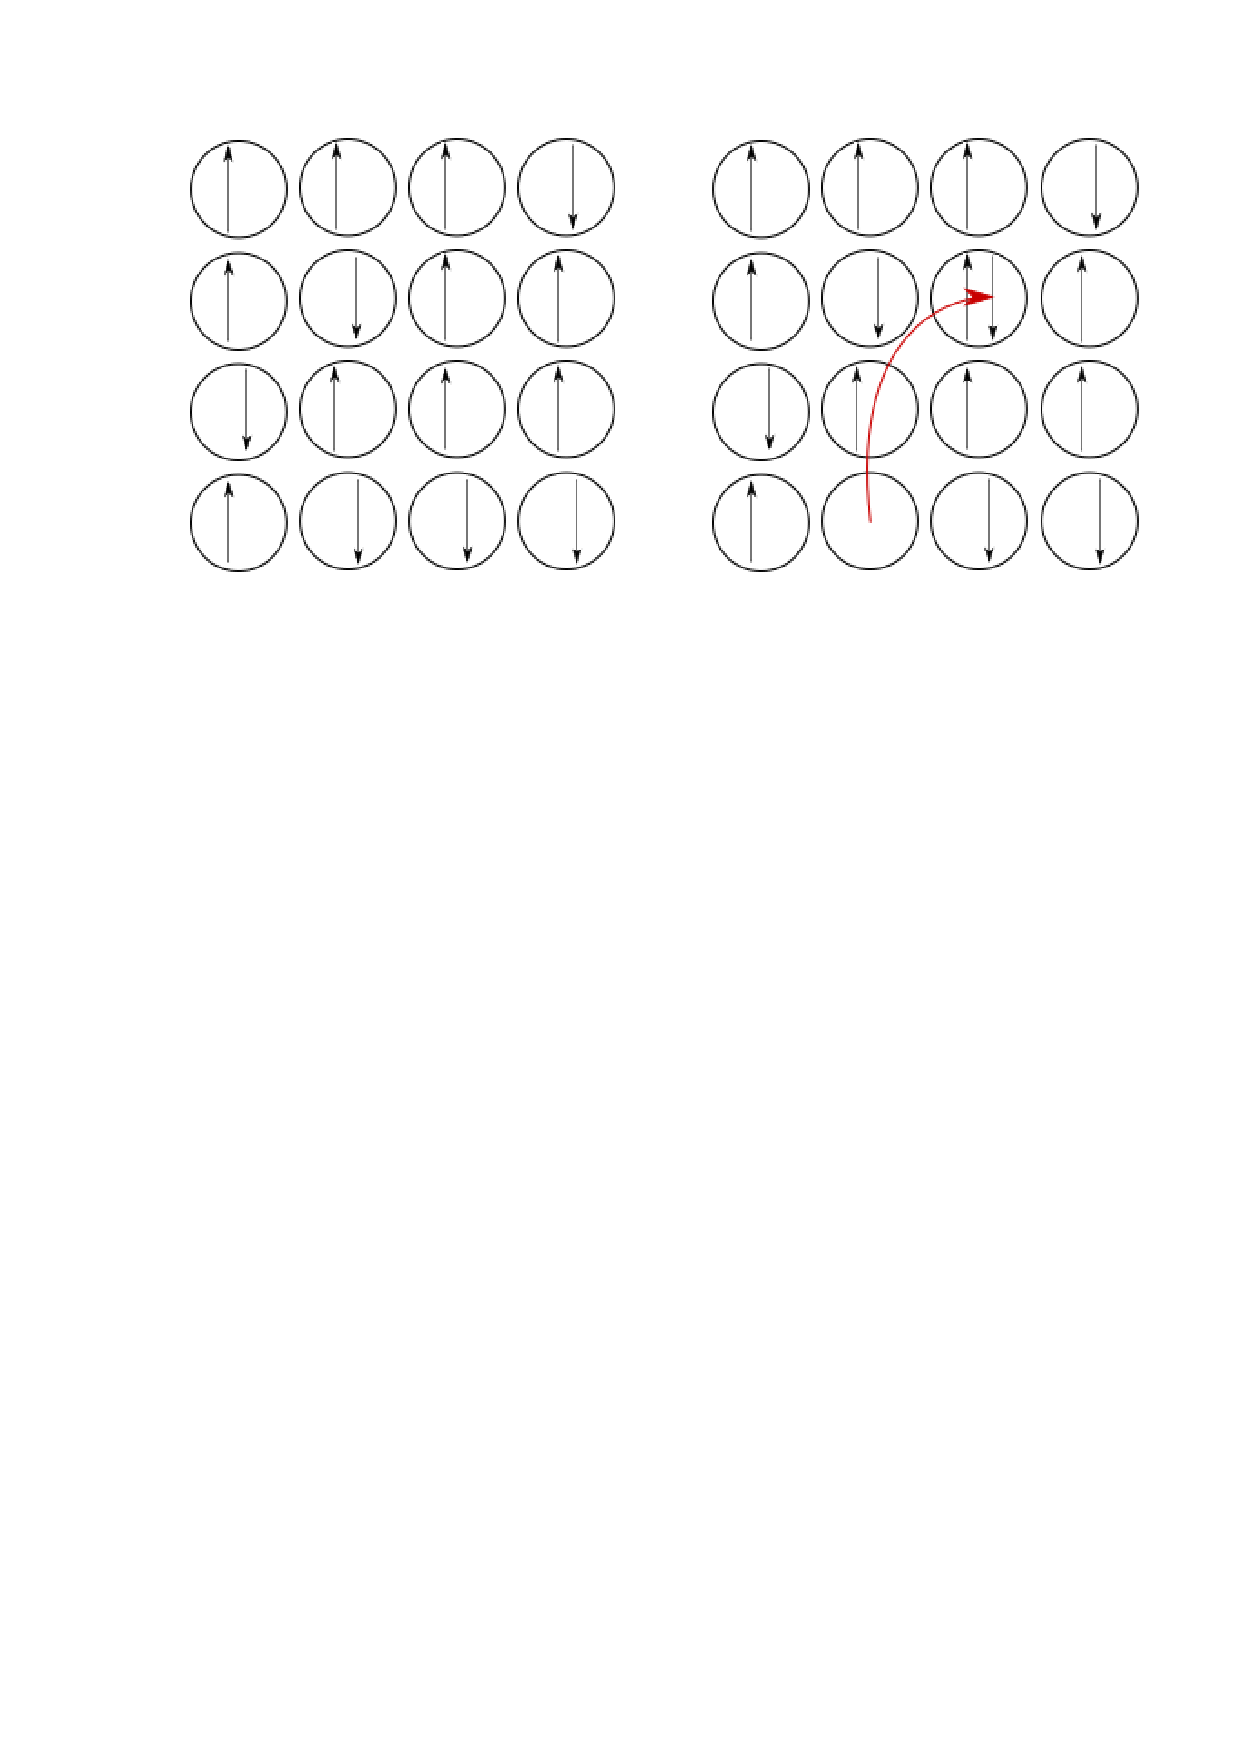
\includegraphics[width = 9cm]{Hubbard/hubbardOneHoleOneDoublyOcV2.png}
\caption[Configuration of the Hubbard model on the square lattice with a hole and a doubly occupied site.]{On the right, a configuration of hydrogen atoms on a square lattice with a hole and a doubly occupied site obtained by delocalization of the spin down electron on the left.}
\end{figure}

If $a$ is large, we have essentially one electron per site at the start.
When an electron is displaced, we end up with a hole and a doubly occupied site.
The potential energy of such a state is

\begin{equation}
E_{H^-} + E_{H^+} - 2 E_H 
\end{equation}

Due to the Coulomb repulsion between the two electrons in $H^-$, this quantity is strictly positive.
Call it $U > 0$.
On the other hand, the system also has kinetic energy: both the hole and the doubly occupied site can delocalize.
Let $W$ be the bandwidth corresponding to the delocalization of an electron on the lattice.
Both the hole and the doubly occupied will stay at the bottom of the band and gain an energy $W/2$ (assuming that this delocalization is of the same order of magnitude).
The dominant transfer integral $-t$ is between nearest neighbors.
The dispersion relation then reads

\begin{equation}
\varepsilon_{\bm k} = -2 t ( \cos k_x + \cos k_y ) 
\end{equation}

The bandwidth is then $W = 8 t$.
The energy of a configuration with a hole and a doubly occupied site is

\begin{equation}
\Delta_c = U - W ,
\end{equation}
where $U$ is practically independent of the lattice parameter $a$.
The bandwidth $W$, however, depends strongly on $a$.
When $a \gg a_0$, where $a_0$ is the Bohr radius, the transfer integral is exponentially small, because only the exponential tails of the wave functions are relevant.
In this limit, $\Delta_c \approx U$ is a large, positive number, and the system is an insulator.
This type of insulator is called a Mott insulator, and $\Delta_c$ is called the charge gap.
As $a$ decreases, $t$ increases, and there must be a critical value $a_c \sim a_0$, for which $U = W$.
Below this value, the computation of $\Delta_c$ is not valid anymore because the gap cannot be negative.
Thus, there must be a metal-insulator transition.
It is possible to see this transition if we apply enough pressure to a Mott insulator so as to decrease $a$ and increase $t$.
A transition of this type was first seen in the 1970's for $V_2 O_3$\footnote{Of course, the transition is not so easy to describe. We should consider the Hubbard model!
However, this simple argument provides an intuitive picture.}.
There is a fundamental difference between a band insulator and a Mott insulator.
While we must pay an energy $\Delta_c$ to make a charge excitation, there is no cost for making a spin excitation: we can flip the spin of an electron without creating a doubly occupied site.
The fluctuations of both charge and spin due to the electron interactions may then lead to magnetic behavior characteristic of correlated  systems.

\section{Computing the partition function for a quadratic Hamiltonian}
\label{sec:Zquadratic}

Let us start by restating the result we want to prove.

If $\mathcal{H} = \bm c^\dagger \bm H \bm c$, where $\bm H$ is a $N \times N$ Hermitian matrix, then we have that

\begin{equation}\label{eq:apZquadratic}
\text{Tr} \big[ e^{-\beta \mathcal{H} } \big] = \prod_{i=1}^N ( 1 + e^{-\beta \lambda_{i} } ) ,
\end{equation}
where $\lambda_{i}$ are the eigenvalues of $\bm H$. 

We will now prove equation (\ref{eq:apZquadratic}). Without loss of generality, let us consider $\bm H$ to be diagonal. Then, its eigenvalues coincide with the diagonal entries, so that $\bm H = \text{diag}(\lambda_{i} )$. The quadratic Hamiltonian may then be  diagonalized

\begin{equation*}
\mathcal{H} = {\bm c}^\dagger \text{diag} (\lambda_{1}, \lambda_{2}, .., \lambda_{N}) \bm c = \sum_{i=1}^N \lambda_{i} n_{i}
\end{equation*}

We continue by induction. When $N=1$, we have

\begin{equation}
\text{Tr} (e^{-\beta\mathcal{H} } ) = \left\langle 0 \left| e^{-\beta \lambda_{1} n_{1}}  \right| 0 \right\rangle + \left\langle 1 \left| e^{-\beta \lambda_{1} n_{1}}   \right| 1 \right\rangle = 1 + e^{-\beta \lambda_{1} }
\end{equation}

Assuming that for $N-1$:

\begin{equation*}
\text{Tr} \big[ e^{-\beta \sum_{i=1}^{N-1} \lambda_{i} n_{i} } \big] = \prod_{i=1}^{N-1} ( 1 + e^{-\beta \lambda_{i} } )
\end{equation*}
we can compute the trace for $i$ going up to $N$.

\begin{equation*}
\begin{split}
&\text{Tr} \big[ e^{-\beta \sum_{i=1}^{N-1} \lambda_{i} n_{i} } \big] = \sum_{i=1}^{N} \left\langle \psi_1^{\lambda_1} \psi_2^{\lambda_2} ... \psi_N^{\lambda_N} \left| e^{-\beta \sum_{i=1}^N \lambda_{i} n_{i}}  \right| \psi_1^{\lambda_1} \psi_2^{\lambda_2} ... \psi_N^{\lambda_N} \right\rangle \\
&= \sum_{i=1}^{N-1} \bigg( \left\langle \{\psi_i^{\lambda_i}\} 0 \left| e^{-\beta \sum_{i=1}^N \lambda_{i} n_{i}} e^{-\beta \lambda_{N} n_{N}} \right| \{\psi_i^{\lambda_i}\} 0 \right\rangle + \left\langle \{\psi_i^{\lambda_i}\} 1 \left| e^{-\beta \sum_{i=1}^N \lambda_{i} n_{i}} e^{-\beta \lambda_{N} n_{N}} \right| \{\psi_i^{\lambda_i}\} 1 \right\rangle \bigg) \\
&= (1 + e^{-\beta \lambda_{N} } ) \sum_{i=1}^{N-1} \left\langle \{\psi_i^{\lambda_i}\} \left| e^{-\beta \lambda_{i} n_{i}} \right| \{\psi_i^{\lambda_i}\} \right\rangle \\
&= (1 + e^{-\beta \lambda_{N} } ) \prod_{i=1}^{N-1} (1 + e^{-\beta \lambda_{i} } ) \\
&= \prod_{i=1}^{N} (1 + e^{-\beta \lambda_{i} } )
\end{split}
\end{equation*}

To complete the proof we note that for any $\bm H$, there exists a unitary matrix $\bm Q$, such that $\bm Q^T \bm H \bm Q = \bm \Lambda = \text{diag}(\lambda_{i})$. Let $\tilde{\bm c} = \bm Q \bm c$, and $\tilde{n_i} = \tilde{c_i}^\dagger \tilde{c_i}$. Then, we find

\begin{equation*}
\mathcal{H} = \bm c^\dagger \bm H \bm c = \bm \tilde{\bm c}^\dagger \bm \Lambda \tilde{\bm c} = \sum_{i=1}^N \lambda_{i} \tilde{n}_{i}
\end{equation*}

The trace is independent of the choice of basis functions. Thus, we have

\begin{equation*}
\begin{split}
\text{Tr} ( e^{-\beta \mathcal{H} } ) &= \text{Tr} \bigg( \prod_{i=1}^N e^{-\beta \lambda_{i} \tilde{n}_{i} } \bigg) \\
&= \prod_{i=1}^N \bigg( 1 + e^{-\beta \lambda_{i} } \bigg) \quad\quad \qedsymbol
\end{split}
\end{equation*}

\section{Density of states for a 1D tight binding model}
\label{sec:dos1d}

Using the definition of the density of states

\begin{equation}
N ( E ) = \frac{1}{N} \sum_{\bm k} \delta_{E,\varepsilon_{\bm k}} \rightarrow \frac{1}{(2\pi)^d} \int d\bm k \, \delta ( E - \varepsilon_{\bm k})\,\, \text{when}\,\, N\rightarrow \infty.
\end{equation}
with $\varepsilon_k = - 2 t \cos k$, in the thermodynamic limit we obtain

\begin{equation}
N ( E ) = \frac{1}{2\pi} \int d k \, \delta ( E + 2t \cos k)
\end{equation}

Now we use a well known property of the delta function

\begin{equation}
\delta ( g(x) ) = \sum_{ \{i | g(x_i) = 0\} } \frac{\delta ( x - x_i) }{| g' ( x_i) |}
\end{equation}

Noting that $g'(k) = - 2 t \sin k$, and that the roots of $g$ (there are two in the first Brillouin zone, to which the integral is restricted) satisfy $\cos k_i = - E / 2t$, so that $\sin k_i = \pm \sqrt{1 - E^2 / 4 t^2}$, we obtain

\begin{equation}
\delta ( E + 2 t \cos k) = \frac{1 }{ \sqrt{4t^2 - E^2 }} \bigg( \delta ( k - k_1 ) + \delta ( k - k_2 ) \bigg)
\end{equation}
leading to the sought result

\begin{equation}
N ( E )_{1d} = \frac{1}{\pi \sqrt{4 t^2 - E^2}}
\end{equation}

\section{Obtaining an effective Heisenberg Hamiltonian as the atomic,  $U/t \gg 1$ limit of the Hubbard model}
\label{sec:heisenberg}

To obtain the effective Hamiltonian corresponding to the $U/t \gg 1$ limit of the Hubbard model to second order in degenerate perturbation theory, we start with its general form, as obtained in equation (\ref{eq:degPert}).

\begin{equation}
\mathcal{H}_{\text{eff}} = - \mathcal{H}_0 \frac{\sum_j n_{j,\sigma} n_{j, -\sigma}}{U} \mathcal{H}_0
\end{equation}

For each element $j$ of the sum, only terms of the type 

\begin{equation*}
\sum_{i(j)} c_{j,\sigma}^\dagger c_{i,\sigma} 
\end{equation*}
contribute.
Here $\sum_{i(j)}$ is a sum over the set of neighbors $i$ of site $j$.

A term of the effective Hamiltonian $\mathcal{H}_{\text{eff}}$ corresponding to the j-th element in the sum reads

\begin{equation*}
-\frac{t^2}{U} \sum_{i(j), \sigma_1, \sigma_2 } c_{i,\sigma_1}^\dagger c_{j,\sigma_1} n_{j,\sigma} n_{j, -\sigma} c_{j, \sigma_2}^\dagger c_{i, \sigma_2}
\end{equation*}

There are only four cases in which the contribution of a term of this type is nonzero.

\begin{itemize}

\item $\sigma = \sigma_1 = \sigma_2$

The operator in the sum then becomes

\begin{equation*}
c_{i,\sigma}^\dagger c_{j,\sigma} n_{j,\sigma} n_{j, -\sigma} c_{j, \sigma}^\dagger c_{i, \sigma} = n_{i,\sigma} n_{j, -\sigma} c_{j,\sigma} n_{j, \sigma} c_{j, \sigma}^\dagger
\end{equation*}

Now, we use a fermionic operator identity:

\begin{equation*}
\begin{split}
&c n = c c^\dagger c = ( 1 -  c^\dagger c ) c = c \\
&\implies c_{j,\sigma} n_{j,\sigma} c_{j,\sigma}^\dagger = c_{j,\sigma} c_{j,\sigma}^\dagger = 1 - n_{j,\sigma}
\end{split}
\end{equation*}

The term of the Hamiltonian corresponding to this first case then takes on the form

\begin{equation*}
n_{i,\sigma} n_{j,-\sigma} ( 1 - n_{j, \sigma} )
\end{equation*}

We can further simplify this term by noting that in the subspace where $\mathcal{H}_{\text{eff}}$ acts, every site is occupied by only a single electron so that

\begin{equation*}
n_{j,\sigma} + n_{j,-\sigma} = 1 \iff 1 - n_{j,\sigma} = n_{j,-\sigma}
\end{equation*}

Since, for fermions we have that $\hat{n} = \hat{n}^k$, whichever the power $k \in \mathbbm{N}$, the final form of the sought term of the Hamiltonian is

\begin{equation*}
n_{i,\sigma} n_{j, -\sigma}
\end{equation*}

\item $-\sigma = \sigma_1 = \sigma_2$

The contribution to the Hamiltonian is exactly of the same form but making $\sigma \mapsto -\sigma$:

\begin{equation*}
n_{i,-\sigma} n_{j, \sigma}
\end{equation*}

\item $\sigma = - \sigma_1 = \sigma_2$

We can use the same reasoning as we did for the first term to obtain

\begin{equation*}
\begin{split}
&c_{i,-\sigma}^\dagger c_{j,-\sigma} n_{j,\sigma} n_{j, -\sigma} c_{j, \sigma}^\dagger c_{i, \sigma} \\
=& c_{i, -\sigma}^\dagger c_{i,\sigma} \underbrace{c_{j,-\sigma} n_{j, -\sigma}}_{c_{j,-\sigma}} \underbrace{n_{j, \sigma} c_{j, \sigma}^\dagger}_{c_{j,\sigma}^\dagger} \\
=& - c_{i, -\sigma}^\dagger c_{i,\sigma} c_{j, \sigma}^\dagger c_{j,-\sigma}
\end{split}
\end{equation*}

\item $-\sigma = - \sigma_1 = \sigma_2$

Analogously, the contribution to the Hamiltonian is

\begin{equation*}
\begin{split}
&c_{i,\sigma}^\dagger c_{j,\sigma} n_{j,\sigma} n_{j, -\sigma} c_{j, -\sigma}^\dagger c_{i, -\sigma} \\
=& - c_{i, -\sigma}^\dagger c_{i,\sigma} c_{j, \sigma}^\dagger c_{j,-\sigma}
\end{split}
\end{equation*}

\end{itemize}

Grouping all these four terms, we obtain

\begin{equation}
\mathcal{H}_{\text{eff}} = \frac{2t^2}{U} \sum_{\left\langle i, j \right\rangle, \sigma} ( - n_{i,\sigma} n_{j,-\sigma} + c_{i,-\sigma}^\dagger c_{i,\sigma} c_{j,\sigma}^\dagger c_{j,-\sigma} ) ,
\end{equation}
where the factor of 2 appears because for each pair of nearest neighbors $\left\langle i, j \right\rangle$, a term comes from the term $n_{j,\sigma} n_{j,-\sigma}$ of the sum $\sum_j n_{j,\sigma} n_{j,-\sigma}$, and another term from $n_{i,\sigma} n_{i,-\sigma}$.

Recall the second quantized form of the spin operators:

\begin{equation}
\begin{cases}
S_i^z = \frac{1}{2} ( n_{i,\uparrow} - n_{i,\downarrow} ) \\
S_i^+ = c_{i,\uparrow}^\dagger c_{i,\downarrow} \\
S_i^- = c_{i,\downarrow}^\dagger c_{i,\uparrow}, \\
\end{cases}
\end{equation}

Using these relations and that the density operator is $n_i = n_{i,\uparrow} + n_{i,\downarrow}$, the following relations hold

\begin{equation}
\begin{split}
S_i^z S_j^z - \frac{1}{4} n_i n_j &= -\frac{1}{2} ( n_{i,\uparrow} n_{j,\downarrow} + n_{i,\downarrow} n_{j,\uparrow} ) \\
S_i^+ S_j^- + S_i^- S_j^+ &= c_{i,\uparrow}^\dagger c_{i,\downarrow} c_{j,\downarrow}^\dagger  c_{j,\uparrow} +  c_{i,\downarrow}^\dagger c_{i,\uparrow} c_{j,\uparrow}^\dagger  c_{j,\downarrow}
\end{split}
\end{equation}

Thus, we may rewrite the effective Hamiltonian:

\begin{equation}
\mathcal{H}_{\text{eff}} = \frac{4t^2}{U} \sum_{\left\langle i, j \right\rangle} \bigg( S_i^z S_j^z - \frac{1}{4} n_i n_j + \frac{1}{2} ( S_i^+ S_j^- + S_i^- S_j^+ ) \bigg)
\end{equation}

But $S_i^z S_j^z + \frac{1}{2} ( S_i^+ S_j^- + S_i^- S_j^+) = \bm S_i \cdot \bm S_j$ and $n_i = n_j = 1$ in the ground state subspace, so the effective Hamiltonian becomes

\begin{equation}
\mathcal{H}_{\text{eff}} = \frac{4t^2}{U} \sum_{\left\langle i, j \right\rangle} \bigg( \bm S_i \cdot \bm S_j  - \frac{1}{4}  \bigg),
\end{equation}
which corresponds to the antiferromagnetic Heisenberg model: $\mathcal{H}_{\text{Heis}} = J \sum_{\left\langle i, j \right\rangle} \bm S_i \cdot \bm S_j $, with $J = 4 t^2 / U$.

\section{On the finite temperature Wick's theorem}
\label{sec:wick}

A product of operators containing $k$ factors $c_i^\dagger$ and $n - k$ factors $c_i$ is brought into \emph{normal ordering} by the operator $\mathcal{N}$ (also written $: \,\,:$) defined as

\begin{equation}
\mathcal{N} [ c_1^{(\dagger)} c_2^{(\dagger)} ... c_n^{(\dagger)} ] = :  c_1^{(\dagger)} c_2^{(\dagger)} ... c_n^{(\dagger)}  : \, \equiv ( - 1 )^P c_{i_1}^{\dagger} c_{i_2}^{\dagger} ... c_{i_k}^{\dagger} c_{i_{k+1}} ... c_{i_n} ,
\end{equation}
where $P$ is the parity of the permutation $1, 2, ..., n \mapsto i_1, i_2, ..., i_n$.

It is straightforward to simplify a product of two operators: $C_1 C_2 = \mathcal{N} [ C_1 C_2 ] + \{ C_1^- , C_2^+ \} $, using the anti-commutation rules.
Here $C_i^{\Pm}$ is a combination of fermionic creation (annihilation) operators. 
The last term is a c-number by assumption.
Defining a contraction as $\contraction{}{C}{ {}_1 }{C_2}
C_1 C_2 \equiv C_1 C_2 - \mathcal{N}[ C_1 C_2 ]$, we obtain $\contraction{}{C}{ {}_1 }{C_2}
C_1 C_2 =  \{ C_1^- , C_2^+ \}  $.
The definition of a contraction holds even there are other operators between the two contracted ones $C_{1, 2}$.
Wick's theorem generalizes the resullt for a product of two operators, giving an expression for the product of an arbitrary number of operators.

Let us state the zero temperature version of Wick's theorem for generic operators $C_i= C_i^+ + C_i^-$.

\begin{equation}\label{eq:wickState}
C_1 C_2 ... C_n = \mathcal{N} [ C_1 C_2 ... C_n ] + \sum_{(ij)} \mathcal{N} [ C_1 C_2 ...
\contraction{}{C_i}{...}{C_j}
C_i ... C_j ... C_n ]
+ \sum_{(ij), (lm)} \mathcal{N} [ C_1 C_2 ...
\contraction{}{C}{ {}_i ... C_l ... }{C_j}
C_i ... 
\contraction[2ex]{}{C}{ {}_l ... C_j ... }{C_m}C_l ... C_j ... C_m ... C_n ] + ... ,
\end{equation}
where the first sum is over single contractions of pairs, the second one on double contractions, and so on.
For odd $n$, the last term contains single unpaired operators.
Otherwise, they are just products of contractions, which are c-numbers.

A general rule follows from the fact that the average of a normally ordered operator vanishes in the ground state.
Two-point correlation functions determine all $n$-point correlation functions.
In particular, for the case of 4 operators, using a self-explanatory abbreviated notation:

\begin{equation}
\left\langle gs | 1234 | gs \right\rangle = \left\langle 12 \right\rangle \left\langle 34 \right\rangle - \left\langle 13 \right\rangle \left\langle 24 \right\rangle + \left\langle 14 \right\rangle \left\langle 23 \right\rangle
\end{equation}

Of course, in the finite temperature case, Wick's theorem is not an operator identity because there is no non ambiguous way of defining normal ordering.
However, for non-interacting particles, the thermal average of a product of one-particle operators is still a sum over all possible contractions of pairs.
All that changes is the definition of the contraction, which is now defined in terms of the thermal average of the product of a pair of operators.
Additionally, the theorem generalizes for time-ordered products, simply by replacing the thermal averages of the pair products by time-ordered pair averages.

In particular, for a free theory, the $n$-particle Green's function, defined by the field operators $\hat{\psi} ( x )$,

\begin{equation}
\mathcal{G} ( x_1, x_2, ..., x_n; y_1, y_2, ... y_n ) \equiv \left\langle \mathcal{T} \hat{\psi} ( x_1 ) \hat{\psi} ( x_2 ) ... \hat{\psi} ( x_n ) \hat{\psi}^\dagger ( y_1 ) \hat{\psi}^\dagger ( y_2 ) ... \hat{\psi}^\dagger ( y_n ) \right\rangle
\end{equation}
is determined solely by the set of all one-particle Green's functions.
Here $x$ and $y$ denote both the complete set of quantum numbers describing the system's degrees of freedom, and imaginary time.

Applying Wick's theorem to the set of non-interacting (and thus independent) particles, we obtain

\begin{equation}
\mathcal{G} ( x_1, x_2, ... x_n; y_1, y_2,... y_n ) = \sum_P (- 1 )^P \mathcal{G}^0 ( x_1; y_{i_1} ) \mathcal{G}^0 ( x_2; y_{i_2} ) ... \mathcal{G}^0 ( x_n; y_{i_n} ) ,
\end{equation}
which corresponds to evaluating the determinant of the matrix $\bm G$, defined as $G_{ij} \equiv \mathcal{G}^0 ( x_i ; x_j )$ for $i, j = 1, 2, ..., n$, where the $\mathcal{G}^0$ are the free-particle Green's functions, also called propagators.

\section{Mean field theory and the variational principle}
\label{sec:mftVariational}

In section \ref{sec:hartree-fock}, we derived the Hartree-Fock form of the Hubbard Hamiltonian.
Here we explain how it arises as a mean field theory prone to studying spontaneous symmetry breaking, generally by resorting to a self-consistent procedure.
This is useful as a first approach to investigate the tendency towards long range ordering, for example in ferromagnetic, or antiferromagnetic phases.

The starting point is the Gibbs-Bogoliubov-Feynman (GBF) inequality

\begin{equation}\label{eq:gibbs}
\mathcal{F} \le \left\langle \mathcal{H} \right\rangle_{\text{MF}} - T \mathcal{S}_{\text{MF}} ,
\end{equation}
which is saturated when $\mathcal{H}_{\text{MF}} = \mathcal{H}$, and in general  serves as a variational principle to find a simpler, non-interacting form for the Hamiltonian.
$\mathcal{F}$ is the system's free energy, $T$ is the temperature and the mean field averages are computed as per Eq.(\ref{eq:mfAv}), while the entropy is computed for the thermal distribution $\rho_{\text{MF}} = e^{-\beta \mathcal{H}_{\text{MF}}}$.
Defining $\mathcal{F}_{\text{MF}} = \left\langle \mathcal{H}_{\text{MF}} \right\rangle_{\text{MF}} - T \mathcal{S}_{\text{MF}}$, we may recast Eq.(\ref{eq:gibbs}) as

\begin{equation}\label{eq:gibbs2}
\mathcal{F} \le \mathcal{F}_{\text{MF}} + \left\langle \mathcal{H} - \mathcal{H}_{\text{MF}} \right\rangle_{\text{MF}} \equiv F
\end{equation}

We seek a quadratic Hamiltonian that minimizes $F$, i.e. $\delta F = 0$.

\begin{equation}
\mathcal{H}_{\text{MF}} = \mathcal{H}_K + \sum_{i, j, \sigma} \varepsilon_{ij} c_{i, \sigma}^\dagger c_{j, \sigma} ,
\end{equation}
and by varying $\varepsilon_{ij}$, we can compute $\delta F$ and show that it is minimized for the mean field Hubbard Hamiltonian in much the same way as we did in section \ref{sec:hartree-fock}.

Although the mean field equations can be obtained both from $\delta \mathcal{F}_{\text{MF}} = 0$ and from $\delta F = 0$, this only means that they both have a vanishing functional derivative at a given (common) configuration of the system.
There may be other configurations at which $\delta \mathcal{F}_{\text{MF}}$ vanishes, but we have only an extremum.
Thus, we must be cautious when analyzing self-consistent solutions to confirm that they  indeed correspond to a minimum of the functional $F$, and not only an extremum of $\delta \mathcal{F}_{\text{MF}}$.

On a final note, we remark that this procedure can be generalized to the \ac{GCE} by considering the GBF inequality for the grand potential:

\begin{equation}\label{eq:gibbsGrand}
\Omega \le \Omega_{\text{MF}} + \left\langle \mathcal{H} - \mathcal{H}_{\text{MF}} \right\rangle_{\text{MF}} \equiv F ,
\end{equation}
where we defined $\Omega_{\text{MF}} = \left\langle \mathcal{H}_{\text{MF}} \right\rangle_{\text{MF}} - T \mathcal{S}_{\text{MF}}- \mu \left\langle \mathcal{N} \right\rangle_{\text{MF}}$, $\mathcal{N}$ being the total number operator.   
		\chapter{Formulating Auxiliary Field Quantum Monte Carlo}
\label{ap:theoAFQMC}

%\pagebreak

\section{Casting the fermionic trace as a determinant}\label{sec:trace_det}

Let the two arbitrary real matrices be $\bm M$ and $\bm N$.
Then, a particular case of the identity (\ref{eq:quadraticIdentity}) is
\begin{equation}\label{eq:particularIdentity}
\Tr \big[ e^{-c_i^\dagger M_{ij} c_j} e^{-c_i^\dagger N_{ij} c_j} \big] = \text{det} ( \bm I + e^{-{\bm M}} e^{-{\bm N}} ) ,
\end{equation}
where a summation over repeated indices is implied, as it wil be throughout this proof.

To prove this identity, we start by proving that
\begin{equation}\label{eq:identity_prod_exps}
e^{-c_i^\dagger M_{ij} c_j}  e^{-c_i^\dagger N_{ij} c_j} = e^{-\sum_\nu c_\nu^\dagger \rho_\nu c_\nu} ,
\end{equation}
where $\lambda_\nu = e^{-\rho_\nu}$ are the eigenvalues of the matrix $e^{-{\bm M}} e^{-{\bm N}}$.

The proof consists of showing that any many-particle state are propagated in the same way when acted upon by any of these two operators, i.e. the LHS operator leads the system to the same state as the RHS operator.

A generic single-particle state reads
\begin{equation}
\left| \phi \right\rangle = \sum_j a_j c_j^\dagger \left| 0 \right\rangle ,
\end{equation}
where $a_j$ are arbitrary coefficients, and $\left| 0 \right\rangle$ is the vacuum state.

Let $\{\left| \mu \right\rangle \}$ be the basis in which the matrix $\bm N$ is diagonal. Using Dirac notation, we then have
\begin{equation}
\bm N = \sum_{\mu} \left| \mu \right\rangle n_\mu \left\langle \mu \right|
\end{equation}

Define new fermionic operators
\begin{equation}\label{eq:changeBasis1}
c_\mu = \sum_j \left\langle \mu | j \right\rangle c_j \quad
c_\mu^\dagger = \sum_j \left\langle j | \mu \right\rangle c_j^\dagger ,
\end{equation}
which may be inverted to obtain
\begin{equation}\label{eq:changeBasis2}
c_j = \sum_\mu \left\langle j | \mu \right\rangle c_\mu \quad
c_j^\dagger = \sum_\mu \left\langle \mu | j \right\rangle c_\mu^\dagger ,
\end{equation}

Now we prove yet another identity that goes into proving equation (\ref{eq:identity_prod_exps}).
\begin{equation}\label{eq:LHS_identity}
e^{-c_i^\dagger N_{ij} c_j} = \prod_\mu \big[ \mathbbm{1} + ( e^{-n_\mu} - 1 ) c_\mu^\dagger c_\mu \big]
\end{equation}
\begin{equation*}
\begin{split}
&\exp({-c_i^\dagger N_{ij} c_j}) = \exp({ - \sum_{\mu\nu} \left\langle \mu | i \right\rangle c_\mu^\dagger N_{ij} \left\langle j | \nu \right\rangle c_\nu }) = \exp({-\sum_{ij}\sum_{ \mu\nu\sigma} \left\langle \mu | i \right\rangle  \left\langle i | \sigma \right\rangle c_\mu^\dagger n_\sigma \left\langle \sigma | j \right\rangle \left\langle j | \nu \right\rangle c_\nu }) , \\
& \text{(using the closure relation} \sum_i \left| i \right\rangle \left\langle i \right|= \mathbbm{1} \text{)} \\
&= \exp({-\sum_{ \mu\nu\sigma} \overbrace{\left\langle \mu | \sigma \right\rangle}^{\delta_{\mu\sigma}}  c_\mu^\dagger n_\sigma \overbrace{\left\langle \sigma | \nu \right\rangle}^{\delta_{\sigma\nu}} c_\nu }) = \exp({-\sum_\mu c_\mu^\dagger n_\mu c_\mu}) = \prod_\mu e^{-n_\mu \hat{n}_\mu} \\
&= \prod_\mu [ \mathbbm{1} + ( - n_\mu \hat{n}_\mu + \frac{n_\mu^2}{2!} \hat{n}_\mu^2 - \frac{n_\mu^3}{3!} \hat{n}_\mu^3 + ... ] = \prod_\mu [ \mathbbm{1} + ( - n_\mu + \frac{n_\mu^2}{2!} - \frac{n_\mu^3}{3!} + ... ) \hat{n}_\mu ] \\
& \text{(since  } \hat{n} = \hat{n}^k \text{  for all  } k \in \mathbb{N} \text{  for fermions since  } n = 0, 1 ) \\
&= \prod_\mu [ \mathbbm{1} + ( e^{-n_\mu} - 1 ) c_\mu^\dagger c_\mu ] \quad\quad \qedsymbol
\end{split}
\end{equation*}

Let 
$
\left| \phi \right\rangle = \sum_j a_j c_j^\dagger \left| 0 \right\rangle
$
be an arbitrary many-particle state. 

Now we use the previous identity to prove that applying the operator of equation (\ref{eq:LHS_identity}) to $\left| \phi \right\rangle$ we obtain
\begin{equation}
e^{-c_i^\dagger N_{ij} c_j} \left| \phi \right\rangle = \sum_j a_j' c_j^\dagger \left| 0 \right\rangle , 
\end{equation}
with
\begin{equation}
a_j' = \sum_{i} (e^{-\bm N})_{ji} a_i
\end{equation}

We start by writing $\left| \phi \right\rangle$ in the basis $\{ \left| \mu \right\rangle \}$ (in which $\bm N$ is diagonal).
\begin{equation}
\left| \phi \right\rangle = \sum_{i,\mu} a_i \left\langle \mu | i \right\rangle c_\mu^\dagger \left| 0 \right\rangle
\end{equation}

Then, we apply the RHS of equation (\ref{eq:LHS_identity}) to $\left| \phi \right\rangle$ written in this basis.
\begin{equation}\label{eq:proofAuxIdentity}
\begin{split}
\sum_\nu \bigg[ \mathbbm{1} + ( e^{-n_\mu} - 1 ) c_\nu^\dagger c_\nu \bigg] c_\mu^\dagger \left| 0 \right\rangle 
&=\bigg[ \mathbbm{1} + ( e^{-n_\mu} - 1 ) c_\mu^\dagger c_\mu \bigg] c_\mu^\dagger \left| 0 \right\rangle \\
&= c_\mu^\dagger \left| 0 \right\rangle + (e^{-n_\mu - 1} - 1) c_\mu^\dagger \left| 0 \right\rangle c_\mu^\dagger e^{-n_\mu} \left| 0 \right\rangle
\end{split}
\end{equation}
\begin{equation}
\begin{split}
&\sum_\nu \bigg[ \mathbbm{1} + ( e^{-n_\mu} - 1 ) c_\nu^\dagger c_\nu \bigg] \left| \phi \right\rangle = \sum_{i\mu} \left\langle \mu | i \right\rangle a_i e^{-n_\mu} c_\mu^\dagger \\
&= \sum_{j\mu i} \left\langle j | \mu \right\rangle e^{-n_\mu} \left\langle \mu | i \right\rangle a_i \left| j \right\rangle = \sum_{j i} \underbrace{\sum_{\mu\nu} \left\langle j | \mu \right\rangle e^{-N_{\mu\nu}} \left\langle \nu | i \right\rangle}_{(e^{-\bm N})_{ji}} a_i \left| j \right\rangle \\
&= \sum_j a_j' c_j^\dagger \left| 0 \right\rangle
\end{split}
\end{equation}

Similarly, by repeating the procedure performing a change of basis to the eigenbasis of $\bm M$, we obtain the more general relation
\begin{equation}\label{eq:propagation_exps}
\begin{split}
&e^{-c_i^\dagger M_{ij} c_j} e^{-c_i^\dagger N_{ij} c_j} \left| \phi \right\rangle = \sum_j a_j'' c_j^\dagger \left| 0 \right\rangle \\
& a_j'' = \sum_i ( e^{-\bm M} e^{-\bm N} )_{ji} a_i
\end{split}
\end{equation}

The amplitude of a propagated state is given by multiplying the initial amplitude by the matrix $e^{-\bm M} e^{-\bm N}$, whichever the basis we choose. Then, since equation (\ref{eq:propagation_exps}) holds in particular for the choice of the eigenbasis of $e^{-\bm M}e^{-\bm N}$ as our basis of single-particle states, if we start with an eigenstate
\begin{equation}
\left| \phi \right\rangle = c_\nu^\dagger \left| 0 \right\rangle ,
\end{equation}
then the amplitude of the propagated state will be given by
\begin{equation}
(e^{-\bm M} e^{-\bm N} )_{\nu\nu} = e^{-\rho_\nu} ,
\end{equation}
the same as we would obtain from equation (\ref{eq:identity_prod_exps}). Clearly, if we start with a state that is an arbitrary combination of states of the eigenbasis, we would obtain the identity (\ref{eq:identity_prod_exps}).

The identity was proven for a single-particle state. Does it generalize to more than one particle? As we did before, we start with propagation by a single factor $e^{-\bm N}$. Take a two-particle state
\begin{equation}
\left| \phi \right\rangle = c_{\mu_1}^\dagger c_{\mu_2}^\dagger \left| 0 \right\rangle
\end{equation}

Now propagate it with $\bm N$, i.e. 
\begin{equation}
\begin{split}
&e^{-c_i^\dagger N_{ij} c_j} \left| \phi \right\rangle = \prod_\mu \bigg[ 1 + (e^{-n_\mu} -1 ) c_\mu^\dagger c_\mu \bigg] c_{\mu_1}^\dagger c_{\mu_2}^\dagger \left| 0 \right\rangle \\
&= e^{-n_{\mu_1}} e^{-n_{\mu_2}} c_{\mu_1}^\dagger c_{\mu_2}^\dagger \left| 0 \right\rangle ,
\end{split}
\end{equation}
where we simply note that by similar reasoning to the previous case, we would in equation (\ref{eq:proofAuxIdentity}) keep two terms corresponding to $\mu_1 \neq \mu_2$. If $\mu_1 = \mu_2$, then both sides are equal to zero due to Pauli's exclusion principle and the equality holds trivially. This reasoning clearly generalizes to an arbitrary superposition of many-particle states. Moreover, we proved the result for a product of two factors $e^{-\bm M} e^{-\bm N}$, but it is also easy to see that by successive changes of basis, we could extend our result to an arbitrary number of factors.

To complete our proof of the identity (\ref{eq:particularIdentity}) that is so crucial in formulating AFQMC, we use the auxiliar identity we just proved (\ref{eq:identity_prod_exps}).
\begin{equation}\label{eq:completeProof}
\begin{split}
&\Tr \bigg[ e^{-\sum_\nu c_\nu^\dagger \rho_\nu c_\nu} \bigg] = \Tr \bigg[ \prod_\nu e^{-c_\nu^\dagger \rho_\nu c_\nu } \bigg] \text{  since  } [\hat{n}_\mu, \hat{n}_\nu] = 0 \\
&= \prod_\nu ( 1 + e^{-\rho_\nu} ) = \text{det} [ \bm I + e^{-\bm M} e^{-\bm N} ], \quad\quad \qedsymbol
\end{split}
\end{equation}
where the last equality stems from the fact that the determinant of a diagonal matrix is just the product of the eigenvalues.

\section{Rank-one updates of the Green's function}\label{sec:greenUpdate}

Consider two matrices $\bm A_1$, $\bm A_2$ written in the form
\begin{equation}
\bm A_{1,2} = \bm I + \bm F \bm V_{1,2} ,
\end{equation}
where $\bm F$ is some matrix. $\bm V_{1,2}$ are diagonal and non-singular and differ only in the $(1,1)$ entry, so that
\begin{equation}
\bm V_1^{-1} \bm V_2 = \bm I + \alpha_1 \bm e_1 \bm e_1^T ,
\end{equation}
where $\bm e_1$ is a vector corresponding to the first column of the identity matrix $\bm I$, and
\begin{equation}
\alpha_1 = \frac{V_2(1,1)}{V_1(1,1)} - 1
\end{equation}

Then, $\bm A_2$ is clearly a rank-one update of $\bm A_1$.
\begin{equation}\label{eq:a2}
\begin{split}
\bm A_2 &= \bm I + \bm F \bm V_1 + \bm F \bm V_1 ( \bm V_1^{-1} \bm V_2 - \bm I ) \\
&= \bm A_1 + \alpha_1 ( \bm A_1 - \bm I ) \bm e_1 \bm e_1^T \\
&= \bm A_1 [ \bm I + \alpha_1 ( \bm I - \bm A_1^{-1} )\bm e_1 \bm e_1^T ]
\end{split}
\end{equation}

To find an expression for the ratio of the determinants of $\bm A_1$ and $\bm A_2$, we shall need to make use of the Sylvester's determinant identity $\det(\bm I + \bm A \bm B ) = \det (\bm I + \bm B \bm A )$.
To prove it, consider the matrices
\begin{equation}
\bm P =
\begin{pmatrix}
\bm I & - \bm A \\
\bm B & \bm I 
\end{pmatrix}
\begin{pmatrix}
\bm I &  \bm A \\
\bm 0 & \bm I 
\end{pmatrix}
\quad
\bm Q =
\begin{pmatrix}
\bm I &  \bm A \\
\bm 0 & \bm I 
\end{pmatrix}
\begin{pmatrix}
\bm I &  -\bm A \\
\bm B & \bm I 
\end{pmatrix}
\end{equation}

Using the identity $\det ( \bm A \bm B ) = \det ( \bm A ) \det ( \bm B )$ applied to these two matrices, we can clearly see that the determinants of the two matrices coincide, i.e.
\begin{equation}
\det ( \bm P) = \det
\begin{pmatrix}
\bm I & -\bm A \\
\bm B & \bm I
\end{pmatrix}
\det
\begin{pmatrix}
\bm I & \bm A \\
\bm 0 & \bm I
\end{pmatrix}
\quad
\det (\bm Q) = \det
\begin{pmatrix}
\bm I & \bm A \\
\bm 0 & \bm I
\end{pmatrix}
\det
\begin{pmatrix}
\bm I & -\bm A \\
\bm B & \bm I
\end{pmatrix}
\end{equation}

The sought identity is obtained by computing the determinants explicitly.
\begin{equation}
\det ( \bm P ) = \det
\begin{pmatrix}
\bm I & \bm 0 \\
\bm B & \bm I + \bm B \bm A 
\end{pmatrix}
= \bm I + \bm B \bm A 
\quad
\det ( \bm Q ) = \det
\begin{pmatrix}
\bm I + \bm A \bm B & \bm 0 \\
\bm B & \bm I
\end{pmatrix}
= \bm I + \bm A \bm B
\end{equation}

A corollary of Sylvester's identity for any two column vectors: $\text{det}[\bm I + \bm x \bm y^T] = 1 + \bm y^T \bm x$ may be used with $x \mapsto ( \bm I - \bm A_1^{-1} ) \bm e_1$, $y \mapsto \bm e_1$ to write the ratio of the determinants of matrices $\bm A_1$ and $\bm A_2$ as
\begin{equation}\label{eq:efRatio}
r_1 = \frac{\text{det}[\bm A_2]}{\text{det}[\bm A_1]} = 1 + \alpha_1 ( 1 - \bm e_1^T \bm A_1^{-1} \bm e_1 ) ,
\end{equation}
which reduces the computation of the ratio $r_1$ to computing the $(1,1)$ entry of $\bm A^{-1}$.

Now we generalize this idea for a sequence of matrices $\bm A_1, \bm A_2, ..., \bm A_i, ..., \bm A_n$ generated by successive rank-one updates: $\bm A_{i+1} = \bm I + \bm F \bm V_{i+1}, \, i = 1, 2, ..., n-1$, with
\begin{equation}
\bm V_i^{-1} \bm V_{i+1} = \bm I + \alpha_i \bm e_i \bm e_i^T \quad \alpha_i = \frac{\bm V_{i+1}(1,1)}{\bm V_i (1,1)} -1
\end{equation}

That is accomplished by use of the  Sherman-Morrison-Woodbury formula, or simply Woodbury matrix identity:
\begin{equation}
( \bm A + \bm B \bm C \bm D )^{-1} = \bm A^{-1} - \bm A^{-1} \bm B ( \bm C^{-1} + \bm D \bm A^{-1} \bm B )^{-1} \bm D \bm A^{-1} ,
\end{equation}
where $\text{dim}(\bm A) = N \times N $, $\text{dim}(\bm B) = N \times K $, $\text{dim}(\bm C) = K \times K $, $\text{dim}(\bm D) = K \times N $, and $N$ and $K$ are integers.
To prove the identity, we use two simple identities, from which the proof easily follows.
\begin{equation}
\bm B + \bm B \bm C \bm D \bm A^{-1} \bm B = ( \bm A + \bm B \bm C \bm D ) \bm A^{-1} \bm B
\quad\,\,
( \bm A + \bm B \bm C \bm D )^{-1} \bm B \bm C = \bm A^{-1} \bm B ( \bm C^{-1} + \bm D \bm A^{-1} \bm B )^{-1}
\end{equation}
\begin{equation}
\begin{split}
\bm A^{-1} &= ( \bm A + \bm B \bm C \bm D )^{-1} ( \bm A + \bm B \bm C \bm D ) \bm A^{-1} = ( \bm A + \bm B \bm C \bm D )^{-1} ( \bm I + \bm B \bm C \bm D \bm A^{-1} ) \\
&= ( \bm A + \bm B \bm C \bm D )^{-1} + ( \bm A + \bm B \bm C \bm D )^{-1} \bm B \bm C \bm D \bm A^{-1} \\
&= ( \bm A + \bm B \bm C \bm D )^{-1} + \bm A^{-1} \bm B ( \bm C^{-1} + \bm D \bm A^{-1} \bm B ) \bm D \bm A^{-1}
\quad
\qed
\end{split}
\end{equation}

The Woodbury identity applied to Eq.(\ref{eq:a2}) gives an expression for $\bm A_2^{-1}$ as a rank-one update of $\bm A_1^{-1}$.
\begin{equation}\label{eq:greenUpdate}
\begin{split}
\bm A_2^{-1} &= \bm A_1^{-1} - \alpha_1 ( \bm I - \bm A_1^{-1} ) {\underbrace{\bigg[ \bm e_1 + \bm e_1^T \bm A_1^{-1} \alpha_1 (  \bm A_1 - \bm I ) \bigg]}_{\bm e_1 \times, \times \bm e_1 \text{(multiply left and right)}}}^{-1} \bm e_1^T \bm A_1^{-1} \\
&= \bm A_1^{-1} - \alpha_1 ( \bm I - \bm A_1^{-1} ) \bm e_1 \bigg[ 1 + \alpha_1 ( 1 - \bm e_1^T \bm A_1^{-1} \bm e_1 ) \bigg]^{-1} \bm e_1^T \bm A_1^{-1}  \\
&= \bm A_1^{-1} - \frac{\alpha_1}{r_1} \bm u_1 \bm w_1^T ,
\end{split}
\end{equation}
where the operation on the first step does not affect the term in parentheses, and we defined
$
\bm u_1 = (\bm I - \bm A_1^{-1} ) \bm e_1 \quad \bm w_1 = (\bm A_1^{-1})^T \bm e_1
$.

Using Eqs.(\ref{eq:efRatio},\ref{eq:greenUpdate}) successively, we find the updates
\begin{equation}
\begin{split}
r_i &= \frac{\text{det}[\bm A_{i+1}]}{\text{det}[\bm A_{i}]} = 1 + \alpha_i ( 1 - \bm e_i^T \bm A_i^{-1}  \bm e_i ) , \,\, \text{and} \\
\bm A_{i+1}^{-1} &= \bm A_i^{-1} - \frac{\alpha_i}{r_i} \bm u_i \bm w_i^T ,
\end{split}
\end{equation}
where $\bm u_i = (\bm I - \bm A_i^{-1} ) \bm e_i$ and $\bm w_i = (\bm A_i^{-1})^T \bm e_i$.

It is possible to generalize this procedure to compute the inverse of $\bm M_k$ as a rank$-(k-1)$ update of $\bm A_1^{-1}$ to devise a delayed update scheme that is more efficient:
\begin{equation}
\bm M_k^{-1} = \bm M_1^{-1} - \bm U_{k-1} \bm D_k \bm W_{k-1}^T ,
\end{equation}
where
\begin{equation}
\bm U_k = [ \bm u_1 , \bm u_2, ..., \bm u_{k-1} ] \quad \text{and} \quad \bm W = [ \bm w_1, \bm w_2, ..., \bm w_{k-1} ] ,
\end{equation}
and $\bm D_k = \text{diag}(\alpha_1 / r_1, \alpha_2 / r_2, ..., \alpha_{k-1} / r_{k-1})$.

In \cite{yip_note_1986}, precise bounds are given on the conditioning of the matrices obtained via such type of Sherman-Morrison updates.
In practice, if the Green's functions are sufficiently well-conditioned, no precision-related issues arise.
Numerical instabilities may arise when the Green's matrices comprise divergent energy scales, and care must be taken to ensure that the algorithm converges.

\section{Particle-hole symmetry and the sign problem}\label{sec:phsSign}

To a greater or lesser extent, all \acl{QMC} methods are plagued by the sign problem.
If the average of the sign is not too small, i.e. $\left\langle \text{sign} \right\rangle \rightarrow 0$, one can simply take more measurements and increase runs proportionally to $\left\langle \text{sign} \right\rangle^{-2}$ to achieve an accuracy comparable to that of the sign problem-free case.
The case of the square lattice is very special because it can be proven that there is no sign problem at half filling.
This is related to \ac{PHS}.

When approaching other models, one must carry out preliminary studies to evaluate whether the sign problem impedes accurate measurements or not, and to set the chemical potential correctly to get the desired filling of the lattice.
In the following figures we give examples of this procedure for a Hubbard chain and for a \acs{TMD} nanoribbon.

\begin{figure}[H]
\includegraphics[scale = 0.5]{Applications/muVsSign.png}
\includegraphics[scale = 0.5]{Applications/densVsSign.png}
	\caption[Average sign as a function of chemical potential/electron density for a Hubbard chain.]{Average sign as a function of chemical potential/electron density for a Hubbard chain.}
	\label{fig:signMuDens}
\end{figure}
\begin{figure}[H]
\includegraphics[scale = 0.5]{Applications/muDens.png}
\includegraphics[scale = 0.5]{Applications/muSignTMDbeta1.png}
	\caption[Electron density as a function of chemical potential for a Hubbard chain. Average sign as a function of chemical potential for a simulation of a $9 \times 4$ TMD nanoribbon using the minimal model described in chapter 2.]{Left: Electron density as a function of chemical potential for a Hubbard chain.
	Right: Average sign as a function of chemical potential for a simulation of a $9 \times 4$ TMD nanoribbon using the minimal model described in chapter 2 at $\beta = 1$ and $U = 14, 16, 18$.
	The sign problem worsens as $U$ is increased.}
	\label{fig:muSign}
\end{figure}
\begin{figure}[H]
\includegraphics[scale = 0.5]{Applications/densSignTMDbeta1.png}
\includegraphics[scale = 0.5]{Applications/muDensTMDbeta1.png}
	\caption[Average sign as a function of electron density for the minimal Hubbard model of \acs{TMDNR}s. Electron density as a function of chemical potential.]{Left: Average sign as a function of electron density for the minimal Hubbard model of \acs{TMDNR}s. Electron density as a function of chemical potential.}
	\label{fig:densSignmuDens}
\end{figure}
\begin{figure}[H]
\includegraphics[scale = 0.5]{Applications/muSignTMDbeta1.png}
\includegraphics[scale = 0.5]{Applications/signTMDmusSignU16beta2.png}
	\caption[Average sign as a function of chemical potential for the same system, and for a system at lower temperature ($\beta = 2$), and fixed on-site/orbital interaction $U = 16$.]{Average sign as a function of chemical potential for the same system (left), and for a system at lower temperature ($\beta = 2$), and fixed on-site/orbital interaction $U = 16$ (right).}
	\label{fig:muDensU16signDens}
\end{figure}
\begin{figure}[H]
\includegraphics[scale = 0.5]{Applications/signTMDmusDensU16beta2.png}
\includegraphics[scale = 0.5]{Applications/Local-av-sign.png}
	\caption[Electron density as a function of the chemical potential for the $9 \times 4$ \acs{TMD} nanoribbon, with $\beta = 2$ and $U = 16$. Sign of the accepted configuration as a function for a few space-time sweeps of the algorithm.]{Left: Electron density as a function of the chemical potential for the $9 \times 4$ \acs{TMD} nanoribbon, with $\beta = 2$ and $U = 16$.
	Right: Sign of the accepted configuration as a function for a few space-time sweeps of the algorithm, for the same \acs{TMDNR}; the red line is the local average of the sign.}
	\label{fig:SignLoc}
\end{figure}

To prove that the half filled square lattice is sign problem-free we start by invoking two well known identities.
Respectively, for any non-singular matrix $\bm A$, and for symmetric, non-singular matrices $\bm A_{l=1,... m}$:
\begin{equation}\label{eq:identities}
( \bm I + \bm A^{-1} )^{-1}  = \bm I - ( \bm I + \bm A )^{-1} \,\,\,\, \,\,\,\, ( \bm I + \bm A_m^{-1}  \bm A_{m-1}^{-1}  ...  \bm A_{1}^{-1} )^{-1} =  \bm I - [ ( \bm I + \bm A_m \bm A_{m-1} ... \bm A_1 )^{-1} ]^T
\end{equation}

Moreover, given any two matrices $\bm A$ and $\bm B$, there exists a third one $\bm \Pi$, which anti-commutes with $\bm A$, i.e. $ \bm \Pi \bm A  + \bm A \bm \Pi = 0$, and commutes with $\bm B$, i.e. $ \bm \Pi \bm B  - \bm B \bm \Pi = 0$ (or vice-versa).
Then, the following two relations hold:
\begin{equation}
\begin{split}
( \bm I + e^{\bm A - \bm B} )^{-1} &= \bm I - \bm \Pi^{-1} ( \bm I + e^{\bm A + \bm B} )^{-1} \bm \Pi \\
\det [ \bm I + e^{\bm A - \bm B} ] &= e^{\Tr [\bm A - \bm B ]} \det [ \bm I + e^{\bm A + \bm B} ]
\end{split}
\end{equation}

The first is proven by using the first identity of Eq.(\ref{eq:identities}):
\begin{equation}
\begin{split}
( \bm I + e^{\bm A - \bm B} )^{-1} &= \bm I - ( \bm I + e^{-\bm A + \bm B} )^{-1}  = \bm I - ( \bm I + e^{\bm \Pi^{-1} ( \bm A + \bm B) \bm \Pi } )^{-1} \\
&= \bm I - ( \bm I + \bm \Pi^{-1} e^{\bm A + \bm B} \bm \Pi )^{-1} = \bm I - \bm \Pi^{-1} ( \bm I + e^{\bm A + \bm B} )^{-1} \bm \Pi
\end{split}
\end{equation}

The proof of the second uses the commutation relations:
\begin{equation}
\begin{split}
\bm I + e^{\bm A - \bm B} &= e^{\bm A - \bm B} ( \bm I + e^{-(\bm A - \bm B)} ) = e^{\bm A - \bm B} ( \bm I + e^{-\bm A + \bm B} ) \\
&=e^{\bm A - \bm B} ( \bm I + e^{\bm \Pi^{-1} \bm A \bm \Pi +\bm \Pi^{-1} \bm B \bm \Pi  } ) = e^{\bm A - \bm B} ( \bm I + \bm \Pi^{-1} e^{\bm A + \bm B} \bm \Pi ) \\
&= e^{\bm A - \bm B}  \bm \Pi^{-1} ( \bm I + e^{\bm A + \bm B} ) \bm \Pi \\
\rightarrow \det [ \bm I + e^{\bm A - \bm B} ]&= \det [ e^{\bm A - \bm B} ] \det [ \bm \Pi^{-1} ] \det [ \bm I + e^{\bm A + \bm B} ] \det [ \bm \Pi ] \\
&= e^{ \Tr [ \bm A - \bm B ] } \det [ \bm I + e^{\bm A + \bm B} ]
\end{split}
\end{equation}

Similarly, we can prove that for symmetric matrices $\bm A$, $\bm B$, if we can find a non singular matrix $\bm \Pi$ that commutes with $\bm A$ and anti-commutes with $\bm B$, then:  $\det[ \bm I + e^{\bm A} e^{-\bm B} = e^{ \Tr [ \bm A - \bm B ] } \det [ \bm I + e^{\bm A} e^{\bm B} ]$ and
\begin{equation}
(\bm I + e^{\bm A} e^{-\bm B} )^{-1} = \bm I - [\bm \Pi^{-1}]^T [ ( \bm I + e^{\bm A} e^{\bm B} )^{-1} ]^T \bm [\bm \Pi^{-1} ]^T
\end{equation}

This theorem generalizes for the products we use in our code: $\bm M_\sigma = \bm I + e^{\bm A} e^{\sigma \bm B_k} e^{\bm A} e^{\sigma \bm B_{k-1}} ... e^{\bm A} e^{\sigma \bm B_1}$.
If we can find a non singular matrix $\bm \Pi$, such that $\{\bm \Pi, \bm A \} = 0$ and $[ \bm \Pi, \bm B_l] = 0$, then we have
\begin{equation}
\bm M_\downarrow^{-1} = \bm I -[ \bm \Pi^{-1}]^T [\bm M_\uparrow^{-1} ]^T \bm \Pi^T \quad \text{and} \quad \det [ \bm M_\downarrow ] = e^{k \Tr [ \bm A ] - \sum_{l = 1}^k \Tr [ \bm B_l] } \det [ \bm M_\uparrow ]
\end{equation}

Since $\det [ \bm M_\downarrow ] $ is then proportional to $\det [ \bm M_\uparrow ]$, and $e^{k \Tr [ \bm A ] - \sum_{l = 1}^k \Tr [ \bm B_l] }$ is positive, the weight of the classical spin configuration $\det [ \bm M_\uparrow ] \det [ \bm M_\downarrow ] $ will always be positive, and there will be no sign problem.
Now, it turns out that this is only possible at half filling.
Away from half filling, we cannot find a $\bm \Pi$ obeying these conditions.

The matrix $\bm \Pi$ is intimately related to the particle hole transformation.
In fact, for the \acs{1D} chain, or the square lattice, if we take $\bm \Pi_{x (y) } = \text{diag} ( 1, -1, 1, -1, ...)$, then the particle-hole transformation of the Green's function reads
\begin{equation}
\bm G^\downarrow = \bm I - \bm \Pi_x (\bm G^\uparrow)^T \bm \Pi_x \text{  for the chain} \,\, \text{and} \,\, \bm G^\downarrow = \bm I - \bm \Pi (\bm G^\uparrow)^T \bm \Pi \text{  for the square lattice} ,
\end{equation}
where $\bm \Pi = \bm \Pi_x \otimes \bm \Pi_y$, the tensor (Kronecker) product of the two matrices.

This reasoning is not only valid for the chain and square lattice, but actually holds for any bipartite lattice, such as the honeycomb lattice.
Unfortunately, for example for the triangular lattice, it does not.
This makes simulations on the triangular lattice (such as the one in this work) and other non bipartite lattices potentially much harder to control. 
		\cleardoublepage
	\end{appendix}
\end{appendices}


\end{document}